\begin{table*}[ht]
    \footnotesize
    \setlength{\tabcolsep}{0.9mm}
    \centering

  \caption{
Classification results on three variants of the ScanObjectNN~\cite{uy2019revisiting} dataset and the ModelNet40~\cite{wu20153d} dataset, including the number of trainable parameters and overall accuracy (OA). All methods apply default data augmentation as used in~\cite{zhou2024dynamic}. \textcolor{red}{$^*$} indicates reproduced results. For ScanObjectNN~\cite{uy2019revisiting}, results are reported without voting. For ModelNet40~\cite{wu20153d}, results are shown without and with voting, respectively denoted as (-/-).
}
  \vspace{-10pt}
    \begin{tabular}{lcccccccc}
    
    \toprule
    \multirow{2.3}{*}{Method} &\multirow{2.3}{*}{Reference} &\multirow{2.3}{*}{Tunable params. (M)} &\multirow{2.3}{*}{FLOPs (G)} &\multicolumn{3}{c}{ScanObjectNN} &\multicolumn{2}{c}{ModelNet40}\\
		\cmidrule(r){5-7} \cmidrule{8-9}
	& & & &OBJ\_BG & OBJ\_ONLY &PB\_T50\_RS & Points Num. & OA (\%)      \\
    \midrule
    \multicolumn{9}{c}{\textit{Supervised Learning Only}} \\
    \midrule
    PointNet~\cite{qi2017pointnet} & CVPR 17 & 3.5 & 0.5  & 73.3  & 79.2  & 68.0 & 1k & - / 89.2 \\
    PointNet++~\cite{qi2017pointnet++}   & NeurIPS 17 & 1.5 & 1.7 & 82.3  & 84.3  & 77.9 & 1k & - / 90.7\\
    DGCNN~\cite{wang2019dynamic}  & TOG 19 & 1.8 & 2.4 & 82.8  & 86.2  & 78.1 & 1k & - / 92.9 \\
    MVTN~\cite{hamdi2021mvtn}  & ICCV 21 & 11.2 & 43.7 & -     & -     & 82.8 & 1k & - / 93.8\\
    PointNeXt~\cite{qian2022pointnext} & NeurIPS 22  & 1.4 & 1.6 & -     & -  & 87.7 & 1k & - / 94.0\\
    PointMLP~\cite{ma2022rethinking}  & ICLR 22 &  13.2 & 31.4  & -    & -     & 85.4  & 1k & - / 94.5\\
    RepSurf-U~\cite{ran2022surface} & CVPR 22 & 1.5   & 0.8 &  -  & -    & 84.3  & 1k  & - / 94.4 \\
    ADS~\cite{hong2023attention} & ICCV 23 & -  & -  &  - & -   & 87.5 & 1k  & - / 95.1 \\
    \midrule
    \multicolumn{9}{c}{\textit{ Self-Supervised Representation Learning (Full fine-tuning)}} \\
    \midrule
    % Transformer~\cite{} &  & 22.1 & & 79.86 & 80.55 &  77.24 & 1k & 91.4 \\
    OcCo~\cite{wang2021unsupervised} & ICCV 21 & 22.1 & 4.8 & 84.85 & 85.54 & 78.79 & 1k & - / 92.1 \\
    Point-BERT~\cite{yu2022point}  & CVPR 22 & 22.1 & 4.8  & 87.43 & 88.12 &  83.07 & 1k & - / 93.2 \\
    MaskPoint~\cite{liu2022masked} & ECCV 22 & 22.1 & - & 89.70 & 89.30 &  84.60 & 1k & - / 93.8 \\
    Point-MAE~\cite{pang2022masked}  & ECCV 22 & 22.1 & 4.8 & 90.02 & 88.29 & 85.18 & 1k & - / 93.8 \\
    Point-M2AE~\cite{zhang2022point}  & NeurIPS 22 & 15.3 & 3.6 & 91.22 & 88.81 & 86.43 
 & 1k & - / 94.0\\
    ACT~\cite{dong2022autoencoders} & ICLR 23 & 22.1 & 4.8 & 93.29 & 91.91  & 88.21 & 1k & - / 93.7\\
    \recon~\cite{qi2023contrast} & ICML 23& 43.6 & 5.3 & 94.15 & 93.12  & 89.73 & 1k & - / 93.9  \\
    
    \midrule
    \multicolumn{9}{c}{\textit{Self-Supervised Representation Learning (Efficient fine-tuning)}} \\
    
    \midrule
    Point-BERT~\cite{yu2022point} (baseline)  & CVPR 22 & 22.1 (100\%) & 4.8 & 87.43 & 88.12 & 83.07& 1k & {92.7} / {\color{gray}{93.2}}\\
    + IDPT~\cite{zha2023instance}& ICCV 23 & 1.7 (7.69\%) & 7.2 & {88.12}\dplus{+0.69} & {88.30}\dplus{+0.18} & {83.69}\dplus{+0.62} &1k & {92.6}{\dtplus{-0.1}} / {\color{gray}{{93.4}}}{\color{gray}{\ddplus{+0.2}}} \\
    + DAPT~\cite{zhou2024dynamic}& CVPR 24 & 1.1 (4.97\%) & 5.0 & {91.05}\dplus{+3.62} & {89.67}\dplus{+1.55} & {85.43}\dplus{+2.36} &1k & {93.1}{\dplus{+0.4}} / {\color{gray}{{93.6}}}{\color{gray}{\ddplus{+0.4}}} \\
    + PointGST~\cite{liang2024parameter}& Arxiv 24 & \textbf{0.6} (\textbf{2.71}\%) & 5.0 & {91.39}\dplus{+3.96} & {89.67}\dplus{+1.55} & {85.64}\dplus{+2.57} &1k & {93.4}{\dplus{+0.7}} / {\color{gray}{{93.8}}}{\color{gray}{\ddplus{+0.6}}} \\
    + LST~\cite{sung2022lst}& NeurIPS 22 & 0.8 (3.38\%) & - & {89.15}\dplus{+2.72} & {89.50}\dplus{+1.38} & {83.17}\dplus{+0.10} &1k & {92.9}{\dplus{+0.2}} / {\color{gray}{{93.3}}}{\color{gray}{\ddplus{+0.1}}} \\
    \rowcolor{linecolor!40}+ PLT ({ours})& - & \textbf{0.6} (\textbf{2.71}\%) & 5.0 & {91.57}\dplus{+4.14} & {89.85}\dplus{+1.73} & {86.09}\dplus{+3.02} &1k & {93.5}{\dplus{+0.8}} / {\color{gray}{{94.2}}}{\color{gray}{\ddplus{+1.0}}} \\
    \midrule
    Point-MAE~\cite{pang2022masked} (baseline)& ECCV 22 & 22.1 (100\%)& 4.8& 90.02 & 88.29 & {85.18} & 1k & 93.2 / {\color{gray}{93.8}}\\
    + IDPT~\cite{zha2023instance}& ICCV 23 & 1.7 (7.69\%) & 7.2 & {91.22}\dplus{+1.20} & {90.02}\dplus{+1.73} & {84.94}\dtplus{-0.24} &1k & {93.3}{\dplus{+0.1}} / {\color{gray}{{94.4}}}{\color{gray}{\ddplus{+0.6}}} \\
    + Point-PEFT\textcolor{red}{$^*$}~\cite{tang2024point}& AAAI 24 & 0.7 (3.13\%) & - & {90.19}\dplus{+0.17} & {89.50}\dplus{+1.21} & {84.35}\dtplus{-0.83} &1k & {94.2}{\dplus{+1.0}} / ~~-~~~~~~~~~~~~\\
   + DAPT~\cite{zhou2024dynamic}& CVPR 24 & 1.1 (4.97\%) & 5.0 & {90.88}\dplus{+0.86} & {90.19}\dplus{+1.90} & {85.08}\dtplus{-0.10} &1k & {93.5}{\dplus{+0.3}} / {\color{gray}{{94.0}}}{\color{gray}{\ddplus{+0.2}}} \\
    + PPT\textcolor{red}{$^*$}~\cite{zhang2024positional}& Arxiv 24 & 1.1 (4.97\%) & 5.0 & {89.50}\dtplus{-0.52} & {89.50}\dplus{+1.21} & {84.91}\dtplus{-0.27} &1k & {93.7}{\dplus{+0.5}} / ~~-~~~~~~~~~~~ \\
    + PointGST\cite{liang2024parameter}& Arxiv 24 & \textbf{0.6} (\textbf{2.71}\%) & 5.0 & {91.74}\dplus{+1.72} & {90.19}\dplus{+1.90} & {85.29}\dplus{+0.11} &1k & {93.5}{\dplus{+0.3}} / {\color{gray}{{94.0}}}{\color{gray}{\ddplus{+0.2}}} \\
    + LST~\cite{sung2022lst}& NeurIPS 22 & 0.8 (3.38\%) & 5.0 & {89.67}\dtplus{-0.35} & {89.67}\dplus{+1.38} & {82.75}\dtplus{-2.43} &1k & {93.2}{\ddplus{+0.0}} / {\color{gray}{{93.8}}}{\color{gray}{\ddplus{+0.0}}} \\
    \rowcolor{linecolor!40}+ PLT ({ours})& - & \textbf{0.6} (\textbf{2.71}\%) & 5.0 & {90.88}\dplus{+0.86} & {90.02}\dplus{+1.73} & {85.46}\dplus{+0.28} &1k & {93.8}{\dplus{+0.6}} / {\color{gray}{{94.0}}}{\color{gray}{\ddplus{+0.2}}} \\
    \bottomrule
    \end{tabular}%
  
      \label{tab:sota}

\end{table*}%


\section{Experiments}
\label{sec:experiments}
%In this section, we conduct an extensive evaluation of the proposed Point Ladder Tuning (PLT) method across multiple point cloud datasets and tasks \lr{add citation for datasets and tasks here}. Our experiments aim to validate the effectiveness of PLT in achieving high performance while maintaining parameter efficiency, comparing it against state-of-the-art methods to highlight its advantages.

%In this section, we present a comprehensive evaluation of the proposed Point Ladder Tuning (PLT) method across diverse point cloud datasets and tasks \lr{cite datasets and tasks here}, and performed our comparison across various downstream tasks as 3D Object Classification, Few-Shot Learning, 3D Dense Prediction Task. The experimental analysis is designed to assess the efficacy of PLT in attaining competitive performance while preserving parameter efficiency.
%Furthermore, we compare PLT against state-of-the-art approaches to demonstrate its superior performance and computational advantages. An ablation study is also included.

In this section, we conduct a comprehensive evaluation of our proposed Point Ladder Tuning (PLT) method across multiple point cloud datasets~\cite{wu20153d, uy2019revisiting, yi2016scalable, armeni20163d, dai2017scannet} and diverse tasks, including 3D object classification, few-shot learning, cross-domain methods and 3D dense prediction. Our experiments systematically assess PLT's ability to achieve state-of-the-art performance while maintaining parameter efficiency. Through extensive comparisons with existing approaches, we demonstrate PLT's superior performance and computational advantages. Additionally, we present an ablation study to validate the contribution of each key component in our framework.

%\paragraph{Experimental Settings}
To ensure a fair comparison with prior fine-tuning methods~\cite{zha2023instance, zhou2024dynamic}, we maintain identical experimental setups. All experiments were conducted on an NVIDIA GeForce RTX 3090 GPU (24GB) under controlled hardware conditions. During training, we freeze the weights of the pre-trained backbone and fine-tune only a small subset of parameters in the newly introduced modules.

To ensure a comprehensive comparison, we employ three state-of-the-art pre-trained models as baselines: Point-BERT~\cite{yu2022point}, Point-MAE~\cite{pang2022masked}, and ACT~\cite{dong2022autoencoders}. These models represent diverse pre-training paradigms, shown with detailed discussions in the experiment section.

%To evaluate the effectiveness of our proposed method, we adopt three representative pre-trained models—Point-BERT~\cite{yu2022point}, Point-MAE~\cite{pang2022masked}, and ACT~\cite{dong2022autoencoders}—as baselines. 
%These models cover a diverse set of 3D pre-training paradigms and serve as strong foundations for comparison. 
%Point-BERT~\cite{yu2022point} extends the BERT~\cite{devlin2018bert} framework to 3D point clouds by leveraging a masked point modeling strategy. 
%It learns both low-level geometric structures and high-level semantic features by aligning masked point embeddings with discrete tokens generated by a dVAE-based tokenizer~\cite{vahdat2018dvae}. 
%Point-MAE~\cite{pang2022masked} introduces the masked auto-encoder paradigm into point cloud pre-training, where the model reconstructs masked point patches from the visible ones. 
%This encourages the network to capture meaningful latent representations that generalize well to downstream tasks. 
%To mitigate the challenge of limited labeled 3D data, ACT~\cite{dong2022autoencoders} utilizes a cross-modal teacher-student framework. 
%It transfers knowledge from a fine-tuned cross-modal pre-trained teacher to a 3D point cloud learner, enabling the latter to acquire rich semantic representations through distillation.


% \lr{delete or move to corresponding section}
% To comprehensively evaluate our proposed method, we select three state-of-the-art pre-trained models as baselines: Point-BERT~\cite{yu2022point}, Point-MAE~\cite{pang2022masked}, and ACT~\cite{dong2022autoencoders}. These models represent diverse 3D pre-training paradigms, providing robust reference points for comparative analysis.
% Point-BERT~\cite{yu2022point} adapts the BERT framework~\cite{devlin2018bert} to point cloud processing through masked point modeling. The approach employs a dVAE-based tokenizer~\cite{vahdat2018dvae} to generate discrete tokens, enabling simultaneous learning of geometric structures and semantic features through masked embedding alignment.
% Point-MAE~\cite{pang2022masked} implements a masked autoencoder architecture for point cloud pre-training. By reconstructing occluded point patches from visible regions, the model learns transferable latent representations that demonstrate strong generalization across downstream tasks.
% To mitigate the challenge of limited labeled 3D data, ACT~\cite{dong2022autoencoders} utilizes a cross-modal teacher-student framework. It transfers knowledge from a fine-tuned cross-modal pre-trained teacher to a 3D point cloud learner, enabling the latter to acquire rich semantic representations through distillation.
%ACT~\cite{dong2022autoencoders} addresses the limited availability of labeled 3D data through a teacher-student learning approach. The method works by first training a "teacher" model on cross-modal knowledge, then transferring this knowledge to a "student" model that works specifically with 3D point clouds. This knowledge transfer helps the 3D model learn better features even with limited point cloud training data.


\subsection{3D Object Classification}
\label{sec:classification}

The analysis of object classification results on synthetic dataset is detailed in the supplementary materials

% \textbf{Object Classification on Synthetic Dataset.} We conduct experiments on the ModelNet dataset~\cite{wu20153d}, which contains 12,311 clean 3D CAD models spanning 40 categories. Following the protocol in DAPT~\cite{zhou2024dynamic}, we split ModelNet40 into 9,843 training samples and 2,468 testing samples. During training, we applied standard data augmentation techniques, including random scaling and random translation. The training configuration adheres to the settings used for baseline comparisons. Specifically, the AdamW optimizer is utilized with an initial learning rate of $5 \times 10^{-4}$ and a weight decay of 0.05. A cosine learning rate scheduler with a 10-epoch warm-up period is employed. The model is trained for a total of 300 epochs with a batch size of 32. 

% As shown in Tab.~\ref{tab:sota}, without voting, PLT achieves accuracy rates of 93.8\%, 93.5\% and 93.6\% in Point-MAE, Point-BERT and ACT respectively, representing gains of \textbf{0.6\%}, \textbf{0.8\%} and \textbf{0.6\%} over full fine-tuning. When using voting, PLT continues to outperform full fine-tuning, notably improving Point-BERT's accuracy by an additional \textbf{1.0\%}. These results demonstrate the effectiveness of PLT for point cloud classification, as it explicitly models local structures on the original point cloud while jointly leveraging global and local representations to enhance performance.

\textbf{Object Classification on Real-World Dataset.} While most pre-trained point cloud models are trained on synthetic datasets like ShapeNet~\cite{chang2015shapenet}, which consist of clean, uniformly distributed point clouds, real-world point clouds often present additional challenges such as noise, missing data, and diverse distributions. To evaluate performance in these more realistic scenarios, we use the ScanObjectNN dataset~\cite{uy2019revisiting}, which comprises approximately 15k point cloud samples across 15 categories captured in indoor scenes, often containing background interference and occlusions. The training configuration is consistent with those used for ModelNet~\cite{wu20153d}. As shown in Tab.~\ref{tab:sota}, we evaluate PLT on three variants of the ScanObjectNN dataset (OBJ\_BG, OBJ\_ONLY, and PB\_T50\_RS), using Point-BERT~\cite{yu2022point},  Point-MAE~\cite{pang2022masked} and ACT~\cite{dong2022autoencoders} as baselines.

Our PLT method demonstrates notable accuracy improvements over full fine-tuning in all settings, using only 2.71\% of the parameters. 
Specifically, PLT achieves gains of 4.14\%, 1.73\%, and 3.02\% on the three ScanObjectNN variants with Point-BERT. 
Compared to the state-of-the-art model, PointGST~\cite{liang2024parameter}, PLT achieves accuracy improvements of \textbf{0.45\%} on Point-BERT~\cite{yu2022point} and \textbf{0.24\%} on Point-MAE~\cite{pang2022masked} under the most challenging PB\_T50\_RS setting in ScanObjectNN~\cite{uy2019revisiting}, showcasing the robustness and efficiency of our approach in handling real-world noisy and occluded point cloud data. 
Furthermore, PLT exhibits the least performance degradation on the ACT~\cite{dong2022autoencoders} baseline among all point cloud PEFT approaches. 
While other methods suffer from significant accuracy drops, our approach maintains strong performance, underscoring its architectural strength in preserving semantic representations during adaptation. 
Together, these results validate PLT’s superiority in both performance and parameter efficiency in the real scene dataset.

\begin{table}[!t]
  \centering
  \scriptsize
    \setlength{\tabcolsep}{0.7mm}
  \caption{Few-shot learning on ModelNet40\cite{wu20153d}. Overall accuracy (\%)$\pm$the standard deviation (\%) without voting is reported.}
    \begin{tabular}{lccccc}
    \toprule
   \multirow{2.3}{*}{Methods}&\multirow{2.3}{*}{Reference} & \multicolumn{2}{c}{5-way} & \multicolumn{2}{c}{10-way} \\
\cmidrule{3-6}  &        & 10-shot & 20-shot & 10-shot & 20-shot \\
    % \midrule
    % \multicolumn{6}{c}{\textit{with Self-Supervised Representation Learning (Full fine-tuning)}} \\
    % \midrule
    % % OcCo~\cite{wang2021unsupervised} & ICCV 21      & 94.0$\pm$3.6& 95.9$\pm$2.3 & 89.4$\pm$5.1 & 92.4$\pm$4.6 \\
    % % Point-BERT~\cite{yu2022point}  &  CVPR 22    & 94.6$\pm$3.1 & 96.3$\pm$2.7 & 91.0$\pm$5.4 & 92.7$\pm$5.1 \\
    % MaskPoint~\cite{liu2022masked}  &   ECCV 22   & 95.0$\pm$3.7 & 97.2$\pm$1.7 & 91.4$\pm$4.0 & 93.4$\pm$3.5 \\
    % % Point-MAE~\cite{pang2022masked} &   ECCV 22   & 96.3$\pm$2.5 & 97.8$\pm$1.8 & 92.6$\pm$4.1 & 95.0$\pm$3.0 \\
    % Point-M2AE~\cite{zhang2022point} &  NeurIPS 22    & 96.8$\pm$1.8 & 98.3$\pm$1.4 & 92.3$\pm$4.5 & 95.0$\pm$3.0 \\
    % % ACT~\cite{dong2022autoencoders}  & ICLR 23      & 96.8$\pm$2.3 & 98.0$\pm$1.4 & 93.3$\pm$4.0 & 95.6$\pm$2.8 \\
    % VPP~\cite{qi2024vpp} &  NeurIPS 23    & 96.9$\pm$1.9 & 98.3$\pm$1.5 & 93.0$\pm$4.0 & 95.4$\pm$3.1 \\
    % I2P-MAE~\cite{zhang2023learning} &  CVPR 23    & 97.0$\pm$1.8 & 98.3$\pm$1.3 & 92.6$\pm$5.0 & 95.5$\pm$3.0 \\
    % \recon~\cite{qi2023contrast}  & ICML 23      & 97.3$\pm$1.9 & 98.9$\pm$1.2 & 93.3$\pm$3.9 & 95.8$\pm$3.0 \\
    % PointMamba~\cite{liang2024pointmamba} &  NeurIPS 24 & 96.9$\pm$2.0 & 99.0$\pm$1.1 & 93.0$\pm$4.4 & 95.6$\pm$3.2 \\
    % \midrule
    % \multicolumn{6}{c}{\textit{with Self-Supervised Representation Learning (Efficient fine-tuning)}} \\
    \midrule
   Point-BERT~\cite{yu2022point} (baseline) & CVPR 22 &94.6$\pm$3.1 & 96.3$\pm$2.7 & 91.0$\pm$5.4 & 92.7$\pm$5.1 \\
   + IDPT~\cite{zha2023instance} & ICCV 23    & 96.0$\pm$\textbf{1.7}& 97.2$\pm$2.6& 91.9$\pm$4.4& 93.6$\pm$3.5\\
   + DAPT~\cite{zhou2024dynamic} & CVPR 24&95.8$\pm$2.1 &97.3$\pm$1.3 &92.2$\pm$4.3 &94.2$\pm$3.4 \\
   + PointGST~\cite{liang2024parameter}  & Arxiv 24&96.5$\pm$2.4 &97.9$\pm$2.0 &92.7$\pm$4.2 &95.0$\pm$\textbf{2.8} \\
   + LST~\cite{sung2022lst}  & NIPS 22&94.3$\pm$2.6 &97.1$\pm$1.8 &90.6$\pm$4.7 &93.7$\pm$3.7 \\
   \rowcolor{linecolor!40}+ PLT (\textbf{ours}) & -&\textbf{96.9}$\pm$2.0 &\textbf{98.8}$\pm$\textbf{1.1}&\textbf{93.3}$\pm$\textbf{4.0} &\textbf{95.5}$\pm$3.1 \\
    \midrule
    Point-MAE~\cite{pang2022masked} (baseline) &ECCV 22 & 96.3$\pm$2.5 & 97.8$\pm$1.8 & 92.6$\pm$4.1 & 95.0$\pm$3.0\\
   + IDPT~\cite{zha2023instance} &   ICCV 23    & 97.3$\pm$2.1& 97.9$\pm$1.1& 92.8$\pm$4.1& 95.4$\pm$\textbf{2.9}\\
   + DAPT~\cite{zhou2024dynamic} & CVPR 24 & 96.8$\pm$\textbf{1.8}  &  98.0$\pm$1.0 & 93.0$\pm$\textbf{3.5} & \textbf{95.5}$\pm$3.2  \\
   % + PointGST~\cite{liang2024parameter} & Arxiv 24 & \textbf{98.0}$\pm$\textbf{1.8}  &  98.3$\pm$\textbf{0.9} & \textbf{93.7}$\pm$\textbf{4.0} & \textbf{95.7}$\pm$\textbf{2.4}  \\
   + LST~\cite{sung2022lst}  & NIPS 22&96.6$\pm$2.5 &97.5$\pm$1.7 &92.0$\pm$4.4 &94.9$\pm$3.2 \\
   \rowcolor{linecolor!40}+ PLT (\textbf{ours}) & - & \textbf{97.2}$\pm$2.2  &  \textbf{98.9}$\pm$\textbf{0.9} & \textbf{93.2}$\pm$4.2 & \textbf{95.5}$\pm$\textbf{2.9}  \\
   \midrule
   ACT~\cite{dong2022autoencoders} (baseline) & ICLR 23 & 96.8$\pm$2.3 & 98.0$\pm$1.4 & 93.3$\pm$4.0 & 95.6$\pm$2.8\\
   + IDPT~\cite{zha2023instance} &   ICCV 23    & 96.8$\pm$1.9& 98.3$\pm$1.2& 92.5$\pm$4.1& 95.3$\pm$3.3\\
   + DAPT~\cite{zhou2024dynamic} & CVPR 24 & 95.3$\pm$2.8  &  97.1$\pm$1.7 & 89.8$\pm$4.8 & 94.1$\pm$3.6  \\
   + PPT~\cite{zhang2024positional}  & Arxiv 24 & \textbf{97.1}$\pm$2.3 &98.1$\pm$1.8 &91.8$\pm$4.3 &94.9$\pm$3.4 \\
   + PointGST~\cite{liang2024parameter} & Arxiv 24 & 97.2$\pm$1.9  &  98.3$\pm$1.3 & 92.9$\pm$4.2 & 95.7$\pm$\textbf{2.6}  \\
   + LST~\cite{sung2022lst}  & NIPS 22&96.2$\pm$2.6 &98.0$\pm$1.9 &92.6$\pm$4.4 &94.9$\pm$3.4 \\
   \rowcolor{linecolor!40}+ PLT (\textbf{ours}) & - & 96.9$\pm$\textbf{1.8}  &  \textbf{98.9}$\pm$\textbf{1.0} & \textbf{93.4}$\pm$\textbf{4.0} & \textbf{95.9}$\pm$3.1  \\
    \bottomrule
    % \vspace{-12pt}
    \end{tabular}%
  \label{tab:fewshot}%
\end{table}%

\subsection{Few-Shot Learning}
\label{sec:few_shot}

We further evaluate the transferability of PLT in a few-shot learning setting using the ModelNet40~\cite{wu20153d} dataset, which serves as a standard benchmark for assessing the efficiency of data usage in low-resource settings. The training configuration follows that of the 3D object classification task, with the exception that the number of training epochs is set to 150. Following prior works~\cite{zha2023instance, zhou2024dynamic}, we adopt the standard n-way m-shot protocol, where $n \in \{5, 10\}$ and $m \in \{10, 20\}$.

As summarized in Tab.~\ref{tab:fewshot}, our PLT consistently outperforms both full fine-tuning and state-of-the-art PEFT methods across the majority of settings, regardless of the choice of pre-trained backbone (Point-BERT~\cite{yu2022point}, Point-MAE~\cite{pang2022masked}, or ACT~\cite{dong2022autoencoders}). For example, under the 5-way 20-shot setting, our PLT achieves a overall accuracy of 98.8\% with Point-BERT~\cite{yu2022point}, outperforming other methods such as full fine-tuning (\textbf{+2.5\%}) and PointGST~\cite{liang2024parameter} (\textbf{+0.9\%}). These results highlight our PLT's strong capability to generalize under data-scarce conditions and validate its effectiveness in few-shot point cloud learning tasks. This superior performance is primarily attributed to PLT’s ability to explicitly extract hierarchical local features from the original point cloud, thereby introducing a strong inductive bias that enhances generalization during fine-tuning.

In addition to superior accuracy, our PLT also demonstrates improved stability across few-shot settings. As shown in Tab.~\ref{tab:fewshot}, our method yields consistently lower or comparable standard deviations compared to other PEFT baselines. For instance, under the 5-way 20-shot setting, PLT achieves a standard deviation of only $\pm$1.1\% with Point-BERT, outperforming other methods such as LST~\cite{sung2022lst} ($\pm$1.8\%) and PointGST~\cite{liang2024parameter} ($\pm$2.0\%). This trend is observed across multiple configurations, indicating that PLT not only improves mean performance but also reduces performance variance across different settings. Such stability is particularly critical in few-shot learning scenarios, where training data is limited and model robustness becomes more important.

\subsection{Comparison with Cross-domain PEFT Methods}
\label{sec:compare}

We compare our PLT with a broad range of PEFT methods originally proposed for NLP and 2D vision, adapting them to point cloud scenarios. As shown in Tab.~\ref{tab:origin_finetuning}, methods like VPT~\cite{jia2022visual} and Adapter~\cite{houlsby2019parameter} suffer significant accuracy drops when transferred to the 3D domain. For example, VPT~\cite{jia2022visual} leads to a 4.09\% decrease on the challenging PB\_T50\_RS variant compared to full fine-tuning. Similarly, although Adapter~\cite{houlsby2019parameter} achieves moderate gains on OBJ\_ONLY, it performs poorly on more complex tasks.

LST~\cite{sung2022lst} provides competitive performance in specific settings, but its generalization across variants is limited. In contrast, PLT achieves consistently strong results across various challenging scenarios, while tuning only 0.6M parameters, a fraction of the full model size.

Further comparisons in Tab.~\ref{tab:compare} highlight PLT's superiority under parameter-efficient fine-tuning (PEFT) settings. It outperforms all other PEFT methods, including the strongest 3D-specific methods like PointGST~\cite{liang2024parameter} and DAPT~\cite{zhou2024dynamic}, especially on the most difficult variant PB\_T50\_RS.

These findings highlight a fundamental limitation of many cross-domain PEFT methods: they often underperform in 3D settings due to domain gaps and architectural mismatches. Specifically, point cloud data is inherently unordered, sparse, and irregular in structure—characteristics not well captured by PEFT techniques originally designed for grid-like data in 2D vision or sequential data in NLP.

By contrast, our PLT is designed to explicitly address these 3D-specific challenges. It integrates hierarchical local feature extraction through HLN and incorporates both global and multi-scale local cues via adaptive fusion, enabling it to maintain high performance even in data-scarce or structurally complex scenarios. This design not only ensures strong generalization but also introduces a beneficial inductive bias tailored to 3D spatial structures. As a result, PLT emerges as a unified and effective PEFT solution for point cloud classification, striking an optimal balance between efficiency and accuracy.

\begin{table}
\scriptsize
\setlength{\tabcolsep}{1.9mm}
\centering
\caption{Comparisons of parameter efficient transfer learning methods from NLP and 2D Vision on the hardest variant of ScanObjectNN~\cite{uy2019revisiting}. Overall accuracy (\%) without voting is reported. \#TP represents the tunable parameters. \textcolor{red}{$^*$} denotes reproduced results.}
\label{tab:compare}
\begin{tabular}{ lcccc }
\toprule
 Method &Reference& Design for &\#TP (M) & PB\_T50\_RS \\
\midrule
 Point-MAE~\cite{pang2022masked}  &ECCV 22 & - & 22.1 & 85.18  \\
 Linear probing &- & - & 0.3& 75.99\\
 \midrule
  + Adapter~\cite{houlsby2019parameter}&ICML 19 & NLP & 0.9 & 83.93 \\
  + Perfix tuning~\cite{li2021prefix}& ACL 21 & NLP &0.7 & 77.72  \\
  + BitFit~\cite{zaken2022bitfit} & ACL 21 & NLP &0.3 & 82.62    \\
  + LST~\cite{sung2022lst} & NeurIPS 22 & NLP & 0.8 & 82.75\\
  + LoRA~\cite{hu2021lora} & ICLR 22 & NLP & 0.9&  81.74   \\
  % + DEPT~\cite{shi2024dept} & ICLR 24 & NLP & 0.3 & 79.70\\
  + FourierFT~\cite{Gao2024Fourier} & ICML 24 & NLP &0.3 & 78.57\\
  \midrule
  + VPT-Deep~\cite{jia2022visual}&ECCV 22 & 2D &0.4 &  81.09 \\
  + AdaptFormer~\cite{chen2022adaptformer} &NeurIPS 22 & 2D &0.9  & 83.45 \\
  + SSF~\cite{lian2022scaling} & NeurIPS 22 & 2D &0.4  & 82.58\\
  + FacT~\cite{jie2023fact} & AAAI 23 & 2D & 0.5 & 78.76\\
  % + BI-AdaptFormer~\cite{jie2023revisiting} & ICCV 23 & 2D & 0.4 & 83.66\\
  + SCT~\cite{zhao2024sct} & IJCV 24 & 2D & 0.3 & 80.40\\
  \midrule
  + IDPT~\cite{zha2023instance} &ICCV 23 & 3D & 1.7 &84.94\\
  + Point-PEFT\textcolor{red}{$^*$}~\cite{tang2024point} & AAAI 24 & 3D & 0.7 &84.35\\
  + DAPT~\cite{zhou2024dynamic} & CVPR 24 & 3D & 1.1 & 85.08 \\
  + PPT\textcolor{red}{$^*$}~\cite{zhang2024positional} & Arxiv 24 & 3D & 1.1 & 84.91\\
  + PointGST~\cite{liang2024parameter} & Arxiv 24 & 3D & 0.6 & 85.29\\
  % + PointLoRA~\cite{wang2025pointlora} & CVPR 25 & 3D & 0.8 & \textbf{85.53}\\
  \rowcolor{linecolor!40}+ PLT (\textbf{ours}) & - & 3D & 0.6 & \textbf{85.53} \\
\bottomrule
\end{tabular}
\end{table}


\begin{table}
\footnotesize
\setlength{\tabcolsep}{1.6mm}
\centering
\caption{The overall accuracy (\%) for classical fine-tuning strategies on three variants of ScanObjectNN~\cite{uy2019revisiting} is reported. `\#TP’ means the number of tunable parameters. Linear probing indicates head-tuned only.}
\label{tab:origin_finetuning}
\begin{tabular}{ lcccc }
\toprule
Tuning Strategy & \#TP(M) &OBJ\_BG &OBJ\_ONLY & PB\_T50\_RS \\
\midrule
Point-MAE~\cite{pang2022masked} & 22.1 & 90.02 & 88.29 & 85.18 \\
Linear probing & 0.3  & 87.26\dtplus{-2.76} & 84.85\dtplus{-3.44} & 75.99\dtplus{-9.19}\\
\midrule
+ Adapter~\cite{houlsby2019parameter} & 0.9  & 89.50\dtplus{-0.52} & 88.64\dplus{+0.35} & 83.93\dtplus{-1.25}\\
+ VPT~\cite{jia2022visual} & 0.4  & 87.26\dtplus{-2.76} & 87.09\dtplus{-1.20} &81.09\dtplus{-4.09} \\
+ LST~\cite{sung2022lst} & 0.8  & 89.67\dtplus{-0.25} & 89.67\dplus{+1.38} &82.75\dtplus{-2.43} \\
\bottomrule
\end{tabular}
\end{table}

\subsection{3D Dense Prediction Task}
For dense prediction tasks, including part segmentation and semantic segmentation, we adopt a prediction head similar to that of PointNext~\cite{qian2022pointnext}, allowing us to effectively utilize multi-resolution information and enhance performance while maintaining a low number of trainable parameters.

We validate the effectiveness of PLT on the ShapeNetPart dataset~\cite{yi2016scalable}, comprising 16,881 samples distributed across 16 object categories and 50 part categories. Training is performed using the AdamW optimizer with a weight decay of 0.05 and a cosine learning rate scheduler. The initial learning rate is set to $2 \times 10^{-4}$, with a warm-up period of 10 epochs. The models are trained for 300 epochs using a batch size of 16. As shown in Tab.~\ref{tab:segmentation}, PLT achieves results comparable to other methods in terms of instance-level mIoU (Inst. mIoU) while achieving notable improvements in class-level mIoU (Cls. mIoU). Specifically, PLT improves Inst. mIoU on PointBERT~\cite{yu2022point} by \textbf{0.5\%} over DAPT~\cite{zhou2024dynamic}, demonstrating its effectiveness in capturing fine-grained details.

\begin{table}
  \centering
  \scriptsize
  \setlength{\tabcolsep}{0.6mm}
  \caption{Part segmentation on the ShapeNetPart~\cite{yi2016scalable}. The mIoU for all classes (Cls.) and for all instances (Inst.) are reported. \#TP represents the tunable parameters. \textcolor{red}{$^*$} denotes reproduced results.}
    \vspace{-10pt}
    \begin{tabular}{lcccc}
    \toprule
    Methods & Reference & \#TP (M)& Cls. mIoU (\%) & Inst. mIoU (\%) \\
    \midrule
    \multicolumn{5}{c}{\textit{Supervised Learning Only}} \\
    \midrule
    PointNet~\cite{qi2017pointnet}  & CVPR 17  &- & 80.39 & 83.7 \\
    PointNet++~\cite{qi2017pointnet++}    & NeurIPS 17 &-  & 81.85 & 85.1 \\
    DGCNN~\cite{wang2019dynamic}  & TOG 19 & - & 82.33 & 85.2 \\
    APES~\cite{wu2023attention} & CVPR 23& - & 83.67 & 85.8\\
    \midrule
    \multicolumn{5}{c}{\textit{ Self-Supervised Representation Learning (Full fine-tuning)}} \\
    \midrule
    % Transformer \cite{} & & 27.09 & 83.42 & 85.1 \\
    OcCo~\cite{wang2021unsupervised}  & ICCV 21 & 27.09 & 83.42 & 85.1 \\
    MaskPoint~\cite{liu2022masked}  & ECCV 22 & - & 84.60 & 86.0 \\
    Point-BERT~\cite{yu2022point}  & CVPR 22 & 27.09 & 84.11 & 85.6 \\
    Point-MAE~\cite{pang2022masked}  & ECCV 22 & 27.06 & 84.19 & 86.1 \\ 
    ACT~\cite{dong2022autoencoders}  & ICLR 23 &  27.06 & 84.66 & 86.1 \\
    \midrule
    \multicolumn{5}{c}{\textit{ Self-Supervised Representation Learning (Efficient fine-tuning)}} \\
    \midrule
    Point-BERT~\cite{yu2022point} (baseline) &  CVPR 22 & 27.09 & 84.11 & 85.6 \\ 
    + IDPT\textcolor{red}{$^*$}~\cite{zha2023instance} & ICCV 23 & 5.69  & 83.50  & 85.3  \\
    + DAPT~\cite{zhou2024dynamic} & CVPR 24 & 5.65  & 83.83 & 85.5 \\
    % + PointGST~\cite{liang2024parameter} & Arxiv 24 & 5.58  & \textbf{83.87} & 85.7 \\
    \rowcolor{linecolor!40}+ PLT (\textbf{ours})& - & \textbf{2.08}  & \textbf{83.85} & \textbf{86.0} \\
    \midrule
    Point-MAE~\cite{pang2022masked} (baseline) &  ECCV 22 & 27.06 & 84.19 & 86.1 \\ 
    + IDPT~\cite{zha2023instance} & ICCV 23 & 5.69  & 83.79  & 85.7  \\
    + DAPT~\cite{zhou2024dynamic} & CVPR 24 & 5.65  & 84.01 & 85.7 \\
    % + PPT~\cite{zhang2024positional} & Arxiv 24 & 5.62  & \textbf{84.07} & 85.7 \\
    % + PointGST~\cite{liang2024parameter} & Arxiv 24 & 5.59  & 83.98 & 85.8 \\
    \rowcolor{linecolor!40}+ PLT (\textbf{ours})& - & \textbf{2.08}  & 83.90 & \textbf{85.9} \\
    \bottomrule
    \end{tabular}
    % \vspace{-10pt}
  \label{tab:segmentation}
\end{table}

To comprehensively evaluate the effectiveness of our proposed PLT framework on dense prediction tasks, we conduct semantic segmentation experiments on two widely adopted large-scale indoor scene datasets: S3DIS~\cite{armeni20163d}and ScanNetV2~\cite{dai2017scannet}, with results summarized in Tab.~\ref{tab:semantic_segmentation}. 

S3DIS~\cite{armeni20163d} is a large-scale indoor scene dataset comprising six areas with a total of 273 million points annotated across 13 categories. Following established practices~\cite{dong2022autoencoders}, Area 5 is recommended for evaluation to provide a more reliable and standardized assessment of performance in semantic segmentation tasks. The model is trained using a cosine learning rate scheduler with an initial learning rate of $2 \times 10^{-4}$. Training is performed over 60 epochs with a batch size of 32, while other configurations are consistent with those used for ShapeNetPart~\cite{yi2016scalable}.

ScanNetV2~\cite{dai2017scannet}is a large-scale benchmark dataset for indoor 3D scene understanding, encompassing a diverse range of environments, from compact residential and office spaces to expansive public and commercial buildings. The dataset comprises 1,513 RGB-D scanned scenes with annotations for 20 semantic categories. Following standard practice~\cite{dai2017scannet}, 1,201 scenes are used for training and 312 scenes for testing.For training, we adopt a cosine annealing learning rate scheduler, with an initial learning rate set to $5 \times 10^{-3}$. The models are trained for 500 epochs using a batch size of 32.

As reported in Tab.~\ref{tab:semantic_segmentation}, PLT consistently achieves superior performance across all baselines and datasets, while maintaining a significantly lower number of tunable parameters (2.04M) compared to full fine-tuning (27.02M for Point-MAE~\cite{pang2022masked}, for example). On S3DIS~\cite{armeni20163d}, PLT outperforms all PEFT competitors under each backbone. When applied to ACT~\cite{dong2022autoencoders} as the backbone, PLT achieves an mAcc of 70.6\% and mIoU of 61.5\%, improving over the closest competitor PPT~\cite{zhang2024positional} by \textbf{2.3\%} in mIoU. Similar trends are observed for Point-MAE~\cite{pang2022masked} and Point-BERT~\cite{yu2022point}, with PLT consistently pushing mIoU to above 61\%, outperforming alternatives such as IDPT~\cite{zha2023instance}, DAPT~\cite{zhou2024dynamic}, and PointGST~\cite{liang2024parameter}.

On the more complex ScanNetV2 dataset~\cite{dai2017scannet}, which demands strong generalization due to its large-scale and real-world variability, PLT again demonstrates robust performance. With the Point-BERT~\cite{yu2022point} backbone, PLT reaches a voxel mIoU (VmIoU) of 48.2\% and point mIoU (PmIoU) of 47.8\%, leading the field in both metrics. Notably, the performance gap between PLT and existing methods becomes more evident here: PLT surpasses DAPT~\cite{zhou2024dynamic} and PointGST~\cite{liang2024parameter} by \textbf{4.5\%} and \textbf{2.0\%} respectively on PmIoU for the Point-BERT~\cite{yu2022point} backbone, further underscoring its strong adaptability in real-world 3D segmentation scenarios.

These results reinforce the effectiveness of PLT as a lightweight and generalizable PEFT framework for 3D semantic segmentation. Compared with recent 3D-specific PEFT methods (e.g., PointGST~\cite{liang2024parameter}, DAPT~\cite{zhou2024dynamic}), PLT delivers consistent improvements across multiple backbones and datasets, achieving higher accuracy with fewer trainable parameters. 

The key to PLT's success lies in its Hierarchical Local Network (HLN), which explicitly captures multi-resolution semantic information from the original point cloud. This design enables the model to retain fine-grained spatial details and encode rich global context during the decoding stage. By incorporating both local and global cues in a structured and resolution-aware manner, HLN provides strong inductive bias and greatly enhances the model's capability in dense 3D scene prediction. Consequently, PLT proves particularly effective in segmentation tasks that demand precise localization and semantic consistency across varying spatial scales.

\begin{table}
  \centering
  \scriptsize
  \setlength{\tabcolsep}{1.2mm}
  \caption{Semantic segmentation on the S3DIS~\cite{armeni20163d} and ScanNetV2~\cite{dai2017scannet}. The
    mean accuracy (mAcc) and mean IoU (mIoU) are reported on the S3DIS. VmIoU and PmIoU represents Voxel mIoU and Point mIoU respectively.
    \#TP represents the tunable parameters.}
    \begin{tabular}{lcccccc}
    \toprule
    Methods & Reference & \#TP (M)& \multicolumn{2}{c}{S3DIS} & \multicolumn{2}{c}{ScanNetV2} \\
    & & & mAcc & mIoU & VmIoU & PmIoU \\
    \midrule
    Point-BERT~\cite{yu2022point} (baseline) &  CVPR 22 & 27.02 & 69.7 & 62.1 & 49.9 & 49.6 \\ 
    + Linear probing & - & 5.20  & 65.9  & 56.0 & 30.3 & 30.1  \\
    + IDPT~\cite{zha2023instance} & ICCV 23 & 5.64  & 66.9  & 57.7 & 33.9 & 33.6  \\
    + DAPT~\cite{zhou2024dynamic} & CVPR 24 & 5.61  & 68.3 & 58.9 & 43.6 & 43.3 \\
    + PPT~\cite{zhang2024positional} & Arxiv 24 & 5.58 & 68.8 & 60.5 & 46.7 & 46.3 \\
    + PointGST~\cite{liang2024parameter} & Arxiv 24 & 5.55  & 68.5 & 59.5 & 46.3 & 45.8  \\
    + LST~\cite{sung2022lst} & NeurIPS 22 & 5.65 & 67.4 & 58.6 & 34.5 & 34.2  \\
    \rowcolor{linecolor!40}+ PLT (\textbf{ours})& - & \textbf{2.04}  & \textbf{69.6} & \textbf{61.1} & \textbf{48.2} & \textbf{47.8}  \\
    \midrule
    Point-MAE~\cite{pang2022masked} (baseline) &  ECCV 22 & 27.02 & 69.9 & 60.8 & 51.2 & 50.8 \\ 
    + Linear probing & - & 5.20  & 63.4  & 52.5 & 30.9 & 30.7 \\
    + IDPT~\cite{zha2023instance} & ICCV 23 & 5.64  & 66.6  & 57.6 & 33.5 & 33.2  \\
    + Point-PEFT~\cite{tang2024point} & ICCV 23 & 5.58  & 66.5  & 56.0 & - & -  \\
    + DAPT~\cite{zhou2024dynamic} & CVPR 24 & 5.61  & 68.2 & 59.3 & 41.1 & 40.7 \\
    + PPT~\cite{zhang2024positional} & Arxiv 24 & 5.58 & 68.7 & 60.4 & 46.2 & 45.8\\
    + PointGST~\cite{liang2024parameter} & Arxiv 24 & 5.55  & 68.4 & 58.6 & 44.6 & 44.2\\
    + LST~\cite{sung2022lst} & NeurIPS 22 & 5.65 & 66.9 & 57.7 & 35.2 & 34.9 \\
    \rowcolor{linecolor!40}+ PLT (\textbf{ours})& - & \textbf{2.04}  & \textbf{70.5} & \textbf{61.5} & \textbf{47.2} & \textbf{46.8} \\
    \midrule
    ACT~\cite{dong2022autoencoders} (baseline) &  ICLR 23 & 27.02 & 71.1 & 61.2 & 50.9 & 50.5 \\ 
    + Linear probing & - & 5.20  & 64.1  & 52.0 & 27.2 & 27.0 \\
    + IDPT~\cite{zha2023instance} & ICCV 23 & 5.64  & 64.9  & 55.2 & 32.1 & 31.9 \\
    + Point-PEFT~\cite{tang2024point} & ICCV 23 & 5.58  & 66.0  & 54.6 & - & - \\
    + DAPT~\cite{zhou2024dynamic} & CVPR 24 & 5.61  & 67.9 & 58.5 & 40.3 & 40.0 \\
    + PPT~\cite{zhang2024positional} & Arxiv 24 & 5.58 & 69.1 & 59.2 & 45.5 & 45.2\\
    + PointGST~\cite{liang2024parameter} & Arxiv 24 & 5.55  & 67.6 & 57.4 & 44.2 & 43.8 \\
    + LST~\cite{sung2022lst} & NeurIPS 22 & 5.65 & 67.6 & 58.3 & 34.0 & 33.7 \\
    \rowcolor{linecolor!40}+ PLT (\textbf{ours})& - & \textbf{2.04}  & \textbf{70.6} & \textbf{61.5} & \textbf{46.9} & \textbf{46.6} \\
    \bottomrule
    \end{tabular}
  \label{tab:semantic_segmentation}
\end{table}


\begin{table}[!t]
\scriptsize
\setlength{\tabcolsep}{4.5mm}
\centering
 % \footnotesize
\caption{The effect of each component of our LST. SSF and DP represent Scale\&Shift Fine-tuning and Dynamic Prompt respectively. The tunable parameters (\#TP) and the overall accuracy (\%) on the hardest variant of ScanObjectNN\cite{uy2019revisiting} are reported.}
\label{tab:part}

\begin{tabular}{ ccccc }
   \toprule
 SSF & DP & HLN &  \#TP (M) & PB\_T50\_RS \\
\midrule
\multicolumn{3}{c}{Full fine-tuning}  &22.1 & 85.18 \\
\multicolumn{3}{c}{Linear Probing}  &0.27 & 75.99 \\
\midrule
&\ding {52} &\ding {52}& 0.49 & 84.52 \\
\ding {52}  & &\ding {52}& 0.60 &84.66 \\
\ding {52}  & & & 0.37 & 83.34\\
\rowcolor{linecolor!40}\ding {52}  &\ding {52} &\ding {52}  & 0.60 & \textbf{85.53} \\
\bottomrule
\end{tabular}
\end{table}

\begin{figure}
    \centering
    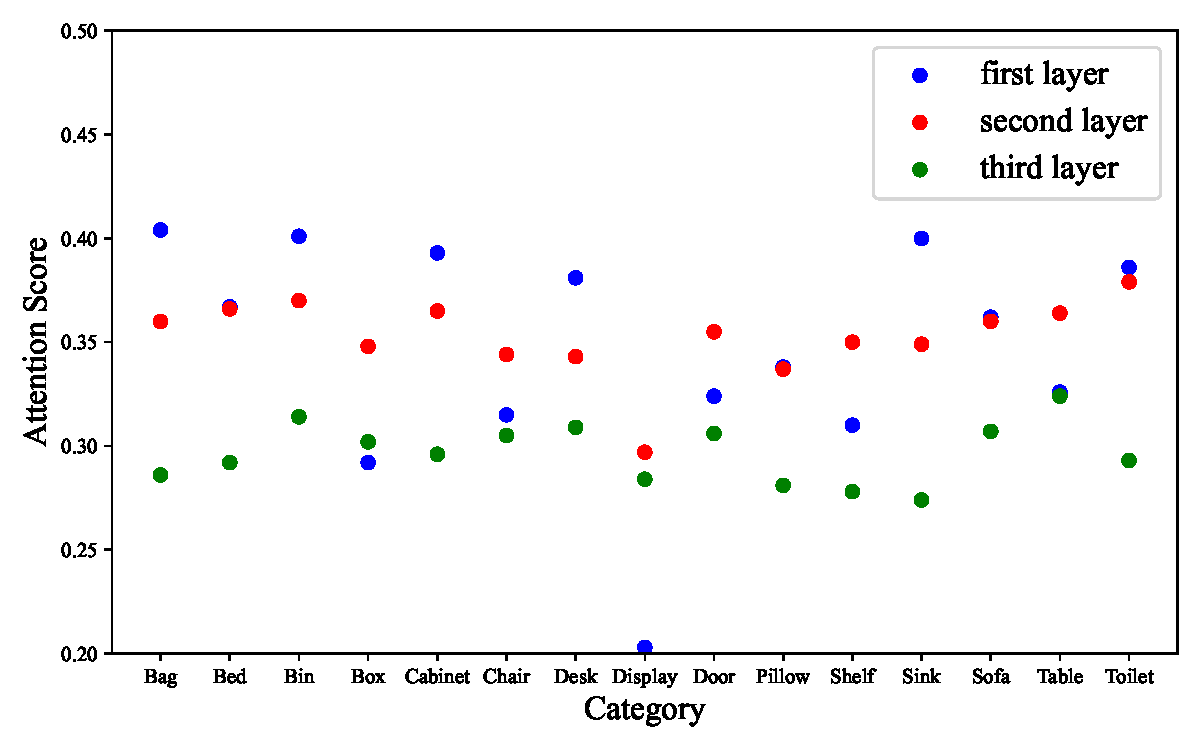
\includegraphics[width=\linewidth]{fig/supplement/hardest.pdf}
    \caption{Local information attention score $z_l$ of LGF. We conduct experiments on ScanObjectNN (PB T50 RS)~\cite{uy2019revisiting} and calculate the average attention score of local information for each category.
}
    \label{fig:attention_score}
    % \vspace{-10pt}
\end{figure}

\begin{table*}
    \centering
    \scriptsize
    \caption{Ablation on hyper-parameters and settings of LST, including the num of neighbors $K$, feature dim $d$ and the num of layers in Hierarchical Ladder Network (HLN). The tunable parameters (\#TP) and the overall accuracy (\%) on the hardest variant of ScanObjectNN\cite{uy2019revisiting} are reported.}
    \label{tab:ablation}
      \vspace{-5pt}
    \resizebox{0.95\linewidth}{!}{
    \begin{subtable}[t]{0.25\linewidth} % 0.245
        \centering
        \scriptsize
         \setlength{\tabcolsep}{1.2mm} % 1.2mm
        \caption{Ablation on $K$ in HLN.}
        \label{tab:k}
        \begin{tabular}{ccc}
           \toprule
            $K$ & \#TP (M) & PB\_T50\_RS \\
            \midrule
            \text{[16, 16, 16]} & 0.60 & 84.46 \\
            \text{[4, 4, 4]} & 0.60 & 84.66 \\
            \text{[4, 8, 16]} & 0.60 & 84.91 \\
            \rowcolor{linecolor!40} \text{[16, 8, 4]} & 0.60 & \textbf{85.46} \\
            \bottomrule
        \end{tabular}
    \end{subtable}

    \begin{subtable}[t]{0.4\linewidth} % 0.235
        \centering
        \scriptsize
         \setlength{\tabcolsep}{1.2mm} % 0.2mm
        \caption{Ablation on $d$ in HLN.}
        \label{tab:dim}
        \begin{tabular}{ccc}
            \toprule
            Feature Dim & \#TP (M) & PB\_T50\_RS \\
            \midrule
            \text{[8, 16, 32, 64]} & 0.46 & 83.17 \\
            \rowcolor{linecolor!40} \text{[16, 32, 64, 128]} & 0.60 & \textbf{85.46} \\
            \text{[32, 64, 128, 256]} & 1.00 & 84.25 \\
            \bottomrule
        \end{tabular}
    \end{subtable}

    \begin{subtable}[t]{0.24\linewidth} % 0.22
    \setlength{\tabcolsep}{1.0mm} % 1.3mm
        \centering
         \scriptsize
        \caption{Ablation on the num of layers.}
        \label{tab:layer}
     
        \begin{tabularx}{\textwidth}{ccc}
            \toprule
            Layer num & \#TP (M) & PB\_T50\_RS \\
            \midrule
            1 & 0.40 & 83.55 \\
            2 & 0.45 & 84.84 \\
            \rowcolor{linecolor!40}3 & 0.60 & \textbf{85.46} \\
            4 & 1.09 & 85.05 \\
            \bottomrule
        \end{tabularx}
    \end{subtable}
}
% \vspace{-10pt}
\end{table*}

\begin{table}[!t]
\scriptsize
\setlength{\tabcolsep}{7.3mm}
\centering
\caption{Fusion way for local and global information in point clouds. The tunable parameters (\#TP) and the overall accuracy (\%) on the hardest variant of ScanObjectNN\cite{uy2019revisiting} are reported.}
\vspace{-10pt}
\label{tab:fusion_way}

\begin{tabular}{ccc}
\toprule
Fusion Way & \#TP (M) & PB\_T50\_RS \\
\midrule
Add & 0.58 & 85.01 \\
Concat & 0.62 & 84.63 \\
Only Global & 0.56 & 84.52 \\
Only Local & 0.56 & 82.86 \\
LGA with Sigmoid & 0.59 & 84.59 \\
\rowcolor{linecolor!40}LGA with Softmax & 0.60 & \textbf{85.46} \\
\bottomrule
\end{tabular}
% \vspace{-10pt}
\end{table}


\begin{table}[!t]
\scriptsize
\setlength{\tabcolsep}{7.8mm}
\centering
\caption{Comparison between HLN and PLT. The tunable parameters (\#TP) and the overall accuracy (\%) on the hardest variant of ScanObjectNN are reported. }
\vspace{-10pt}
\label{tab:sidenet}

\begin{tabular}{ccc}
\toprule
Method & \#TP (M) & PB\_T50\_RS \\
\midrule
Point-MAE & 22.1 & 85.18 \\
% Linear probing & 0.3 & 75.99 \\
HLN & 0.2 & 80.74 \\
\rowcolor{linecolor!40} PLT(Ours) & 0.6 & \textbf{85.46} \\
\bottomrule
\end{tabular}
% \vspace{-15pt}
\end{table}


\subsection{Ablation Study}

\textbf{Effectiveness of PLT Components}. We first investigate the contribution of each individual module in PLT through controlled ablation studies. As shown in Table VII, removing any of the three core components—Scale \& Shift Fine-tuning (SSF), Dynamic Prompt (DP), or the Hierarchical Ladder Network (HLN)—leads to a notable drop in accuracy on the most challenging ScanObjectNN variant (PB\_T50\_RS). As shown in Tab.~\ref{tab:part}, excluding HLN results in a performance decline from 85.53\% to 83.34\%, while excluding SSF or DP alone reduces accuracy to 84.52\% and 84.66\%, respectively. These results clearly demonstrate the complementary roles of all three modules, highlighting that the full integration of SSF, DP, and HLN is essential for maximizing transferability and performance efficiency.

\textbf{Hyperparameter Ablation for Hierarchical Ladder Network.} We conduct a detailed ablation study on the hyperparameters of the HLN, including the number of nearest neighbors $K$, feature dimensions $d$, and the number of hierarchical layers. As summarized in Tab.\ref{tab:ablation}, performance peaks when using $K=[16,8,4]$, feature dimensions $d=[16,32,64,128]$, and a 3-layer architecture, achieving an accuracy of 85.53\% with only 0.60M tunable parameters. This design follows an intuitive hierarchical principle: as the depth of the network increases, the point cloud is progressively downsampled, leading to a reduced number of points in deeper layers. Correspondingly, the number of nearest neighbors $K$ is decreased layer by layer to ensure that neighborhood aggregation remains local and meaningful. If a large $K$ were retained in deeper layers, the receptive field would become overly large relative to the reduced spatial resolution, potentially diluting fine-grained local cues and introducing noise from unrelated distant points. By contrast, using a decreasing neighbor size, such as $K=[16,8,4]$, strikes a balance between capturing sufficient local context in shallow layers and preserving locality in deeper layers. This adaptive design improves the model’s ability to learn multi-scale features across hierarchical levels, leading to superior performance in downstream tasks.

\textbf{Comparison Between HLN and PLT.} To further quantify the value of HLN and its integration within PLT, we compare their standalone performances in Tab.\ref{tab:sidenet}. While HLN alone achieves 80.74\%, integrating it into the full PLT framework improves accuracy to 85.53\%, outperforming even full fine-tuning (85.18\%) with less than 3\% of the tunable parameters. This underscores the importance of coupling lightweight local reasoning structures like HLN with pretrained global backbones for optimal performance.

\textbf{Fusion Strategy for Local and Global Information.} The integration strategy of local and global information plays a critical role in downstream performance. In Tab.~\ref{tab:fusion_way}, we evaluate several fusion mechanisms. The proposed Local-Global Fusion (LGF) with Softmax achieves the highest accuracy (85.53\%), outperforming additive, concatenative, and single-source approaches. Notably, leveraging only local features yields a considerably lower accuracy (82.86\%) than relying solely on global features (84.52\%), reflecting the benefits of pretrained global representation learning.

%\textbf{Attention Score of LGF}. To gain deeper insight into the behavior of LGF, we visualize the local attention weights $s_l$ across categories and network layers in Fig.~\ref{fig:attention_score}. The results reveal three key patterns:
%
%\begin{enumerate}
%    \item The local attention scores are generally lower than 0.5, reaffirming the reliance on pretrained global priors.
%    \item Category-specific variation is more pronounced in early layers and becomes increasingly uniform in deeper layers, suggesting a hierarchical fusion where shallow layers capture category-aware local details while deeper layers consolidate generalized global semantics.
%    \item A downward trend in attention to local features from the first to third layers further supports the notion that the network progressively shifts focus from fine-grained local patterns to more abstract global concepts.
%\end{enumerate}

\textbf{Attention Score of LGF.} Fig.~\ref{fig:attention_score} visualizes local attention weights $s_l$ across categories and layers, revealing three key insights: (1) Scores remain below 0.5, confirming dependence on pretrained global priors; (2) Early layers show strong category-specific variation that diminishes in deeper layers, indicating hierarchical fusion from local details to global semantics; (3) The decreasing attention from first to third layers demonstrates the network's progressive shift from local patterns to abstract concepts.
These findings collectively validate the design of PLT as a lightweight yet powerful PEFT framework for 3D transfer learning, wherein carefully balanced architectural and fusion strategies contribute to superior accuracy and efficiency.

\begin{figure*}
    \centering
    \begin{subfigure}{0.46\textwidth}
        \centering
        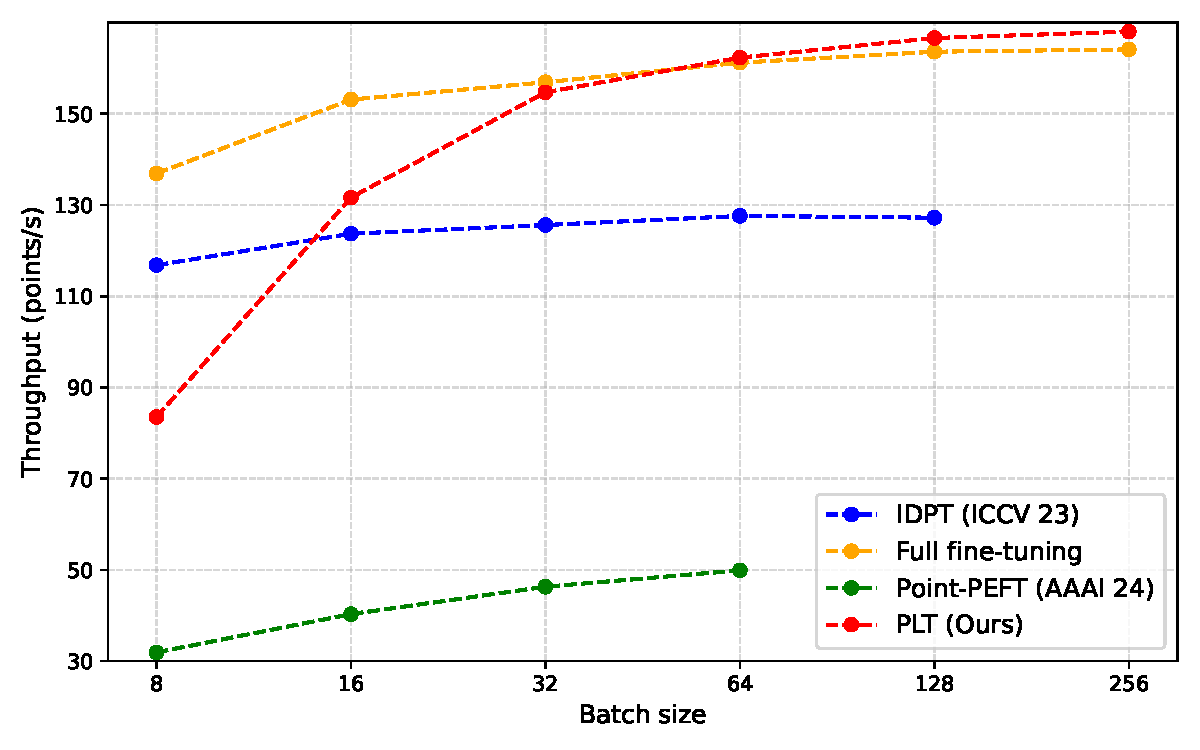
\includegraphics[width=\linewidth]{fig/supplement/performance/train_speed.pdf}
        \caption{Train Speed}
        \label{fig:per1}
    \end{subfigure}
    \hfill
    \begin{subfigure}{0.46\textwidth}
        \centering
        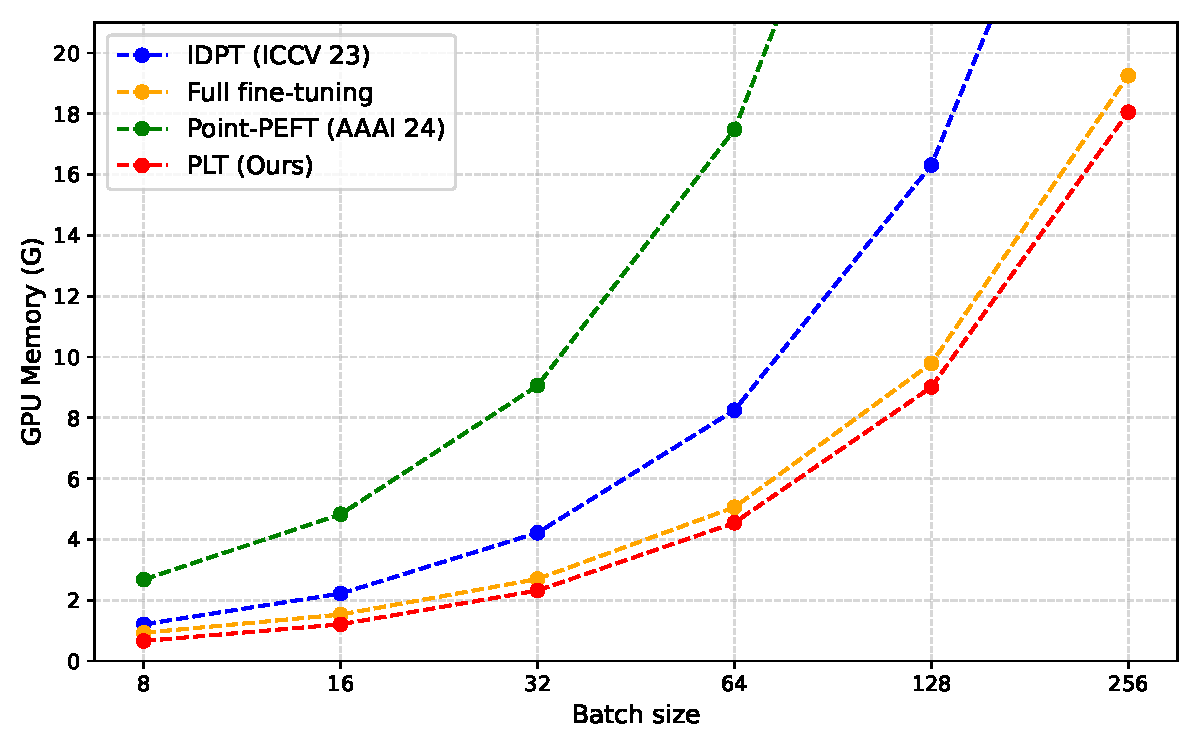
\includegraphics[width=\linewidth]{fig/supplement/performance/train_memory.pdf}
        \caption{Train Memory}
        \label{fig:per2}
    \end{subfigure}
    \hfill
    \begin{subfigure}{0.46\textwidth}
        \centering
        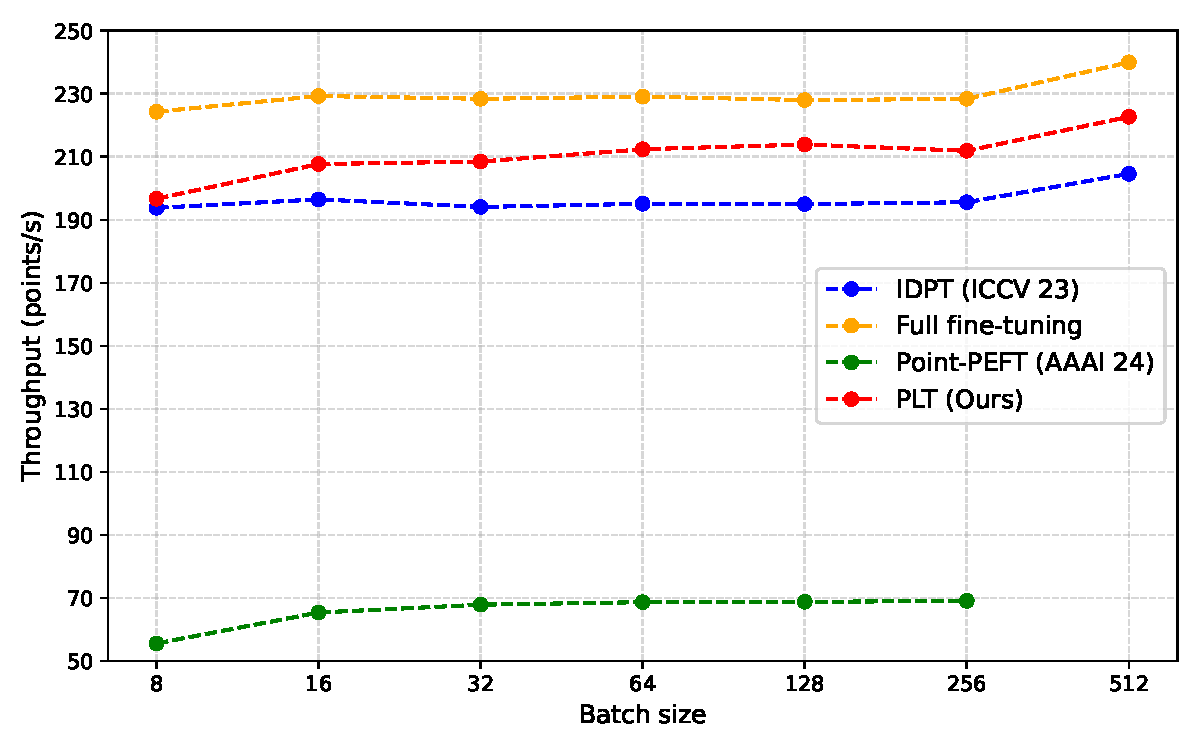
\includegraphics[width=\linewidth]{fig/supplement/performance/infer_speed.pdf}
        \caption{Infer Speed}
        \label{fig:per3}
    \end{subfigure}
    \hfill
    \begin{subfigure}{0.46\textwidth}
        \centering
        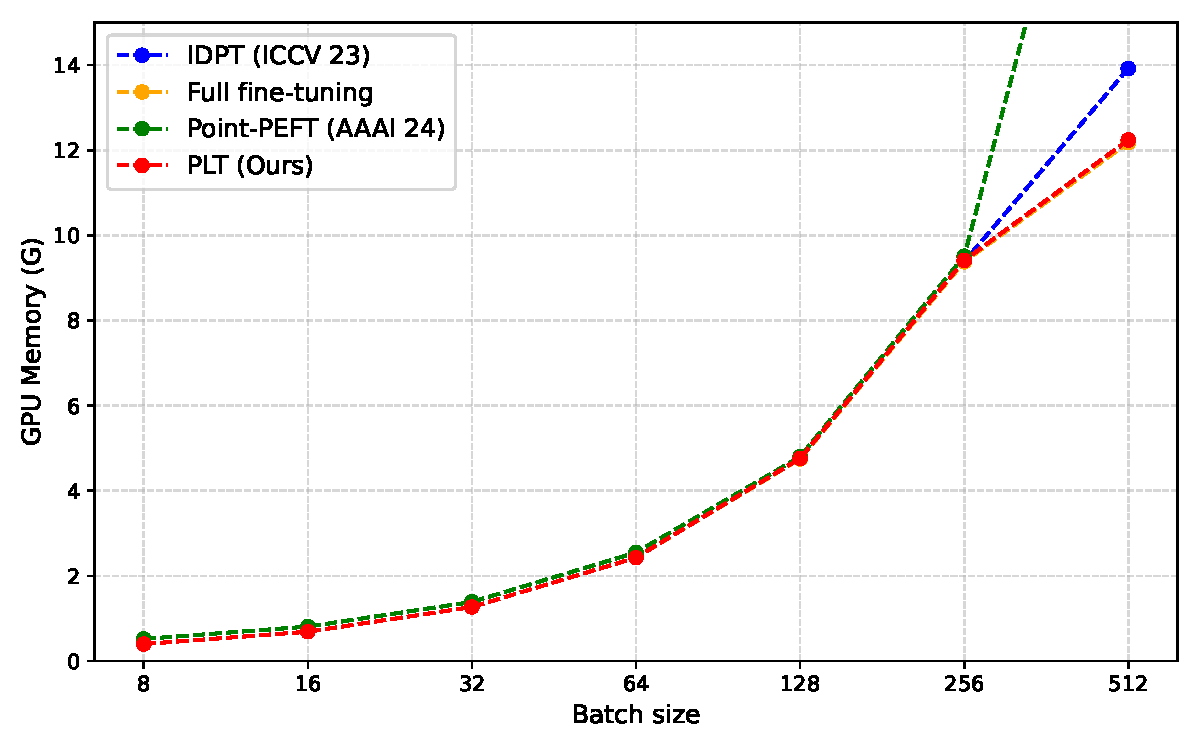
\includegraphics[width=\linewidth]{fig/supplement/performance/infer_memory.pdf}
        \caption{Infer Memory}
        \label{fig:per4}
    \end{subfigure}
    \hfill
    \caption{Comparison of performance between Our PLT and previous methods. We conduct experiments on the hardest variant (i.e., PB\_T50\_RS) of ScanObjectNN~\cite{uy2019revisiting} with Point-MAE baseline~\cite{pang2022masked}. Throughput is measured on a single RTX 3090 GPU.}
    \label{fig:performance}
\end{figure*}

\subsection{Visualization}

\textbf{The Visualization of t-SNE Analysis}. Fig.~\ref{fig:tsne} presents the t-SNE~\cite{van2008visualizing} visualizations of feature manifolds generated by fully fine-tuned methods, point-cloud-specific fine-tuning approaches such as IDPT~\cite{zha2023instance} and DAPT~\cite{zhou2024dynamic}, and our proposed PLT, all trained on the ScanObjectNN PB\_T50\_RS dataset~\cite{uy2019revisiting}. The dispersion of points between categories in the t-SNE plot reflects the quality of the model's feature representation—greater inter-cluster dispersion and smaller intra-cluster average distance indicate stronger discriminative power, facilitating easier classification.

Notably, our PLT demonstrates significantly greater inter-cluster dispersion and a smaller intra-cluster average distance compared to previous works. This suggests that our approach effectively enhances feature separation between categories while maintaining compactness, indicative of a superior ability to represent discriminative features.

Furthermore, PLT achieves these results while using fewer learnable parameters, showcasing its efficiency in leveraging pre-trained models for adaptation to downstream tasks. This not only reduces computational cost but also highlights PLT's potential for broader applicability in resource-constrained environments. In comparison to fully fine-tuned and point-cloud-specific PEFT methods, PLT strikes an optimal balance between parameter efficiency and representation quality, underscoring its value in point cloud learning tasks.

\textbf{Semantic Segmentation Visualizations}. Fig.~\ref{fig:s3dis_1} presents a qualitative comparison of segmentation results between our proposed PLT method and prior fine-tuning approaches in semantic segmentation tasks on Area 5 of the S3DIS dataset~\cite{armeni20163d}. The comparison highlights the advantages of PLT in addressing common challenges in point cloud segmentation. From the first row, it is evident that although full fine-tuning utilizes all model parameters, it often fails to segment object boundaries precisely—leading to blurred edges and misclassification in contiguous areas. This is mainly due to insufficient modeling of local geometric features and lack of multi-scale contextual information.

%A more detailed comparison in the office\_9 scene reveals that methods such as full fine-tuning, IDPT~\cite{zha2023instance}, and DAPT~\cite{zhou2024dynamic} incorrectly classify walls as beams and cluttered regions as ceilings. In contrast, PLT produces more accurate predictions, especially for structural boundaries, owing to its hierarchical local network (HLN), which extracts multi-resolution semantic features and preserves local structural integrity. Similarly, in the office\_35 scene, PLT outperforms other methods in segmenting challenging areas such as the cluttered region and the board. Whereas methods like full fine-tuning, IDPT~\cite{zha2023instance}, and PPT~\cite{zhang2024positional} fail to accurately recognize or segment these regions, PLT demonstrates superior performance, maintaining clarity and precision.

In office\_9, baseline methods (full fine-tuning, IDPT~\cite{zha2023instance}, DAPT~\cite{zhou2024dynamic}) misclassify walls as beams and clutter as ceilings, while PLT achieves accurate boundary segmentation through its hierarchical local network (HLN). This advantage extends to office\_35, where PLT correctly segments challenging areas (clutter, boards) that confuse other methods (PPT~\cite{zhang2024positional}, IDPT). The HLN's multi-resolution feature extraction enables precise structural understanding where conventional approaches fail.

PLT's performance gains stem from its hierarchical feature extraction and local-global fusion. By aggregating multi-resolution features while preserving local details, PLT achieves superior boundary delineation and fine-grained recognition, crucial for 3D scene understanding. Compared to alternatives, PLT delivers: (1) cleaner segmentation with fewer parameters, (2) robust performance across diverse layouts, and (3) precise semantic accuracy, establishing it as an efficient PEFT solution for point cloud segmentation.

%These improvements can be attributed to PLT's hierarchical feature extraction and local-global fusion strategy. By progressively aggregating point features at multiple resolutions and explicitly fusing global context, PLT achieves strong spatial generalization while retaining detail-rich local semantics. This enables it to better delineate object boundaries and differentiate fine-grained structures—key advantages in dense 3D scene understanding.
%In summary, PLT not only achieves visually cleaner and semantically more accurate segmentation results with substantially fewer trainable parameters, but also demonstrates robustness and precision across a wide range of spatial layouts. These qualitative results reinforce PLT's effectiveness and efficiency as a strong PEFT solution for 3D point cloud semantic segmentation.

\begin{figure}
    \centering
    \begin{subfigure}{0.235\textwidth}
        \centering
        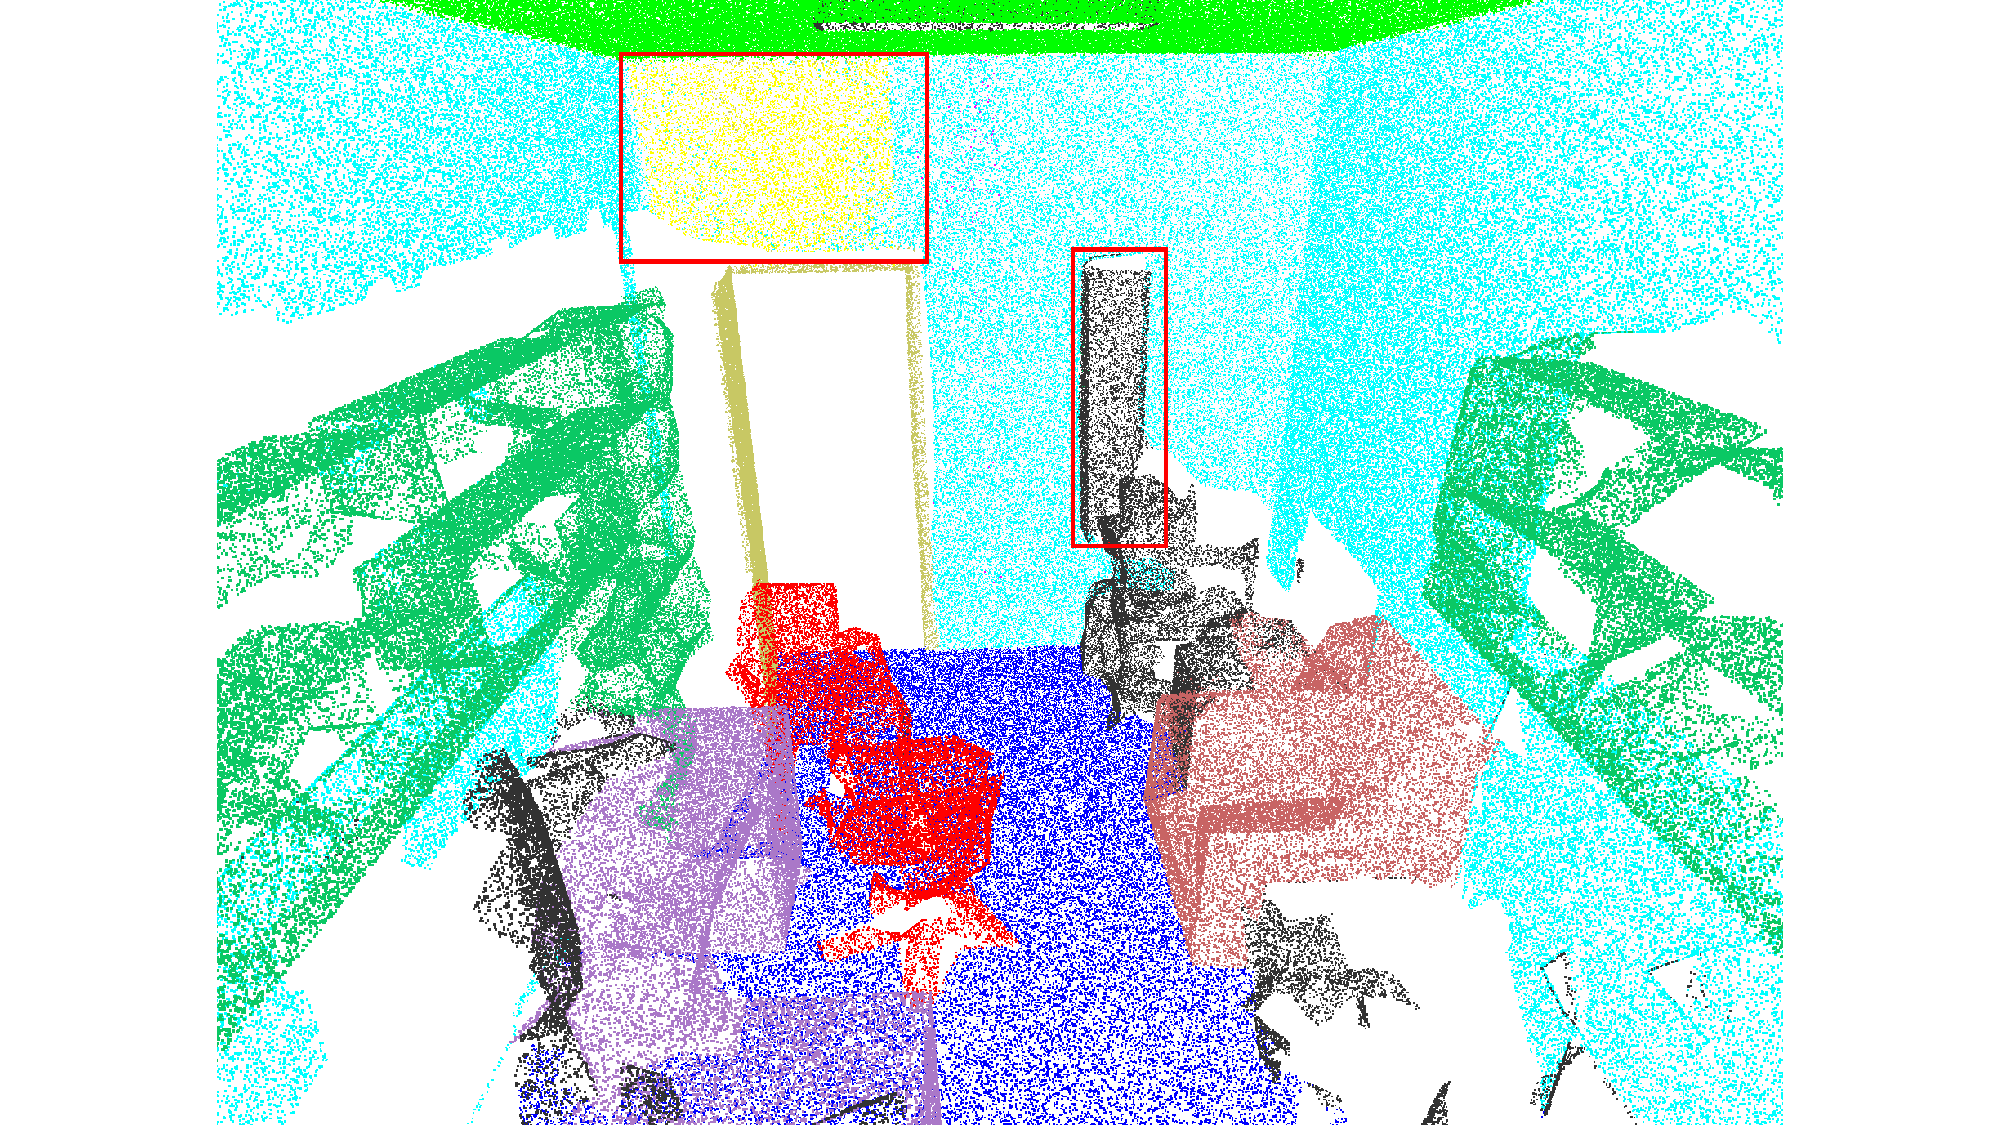
\includegraphics[width=\linewidth]{fig/S3DIS/PointMAE.pdf}
        % \caption*{\textbf{\#TP}:22.1M \textbf{\#OA}:85.18}
        \caption{Full fine-tuning}
        \label{fig:s3dis1}
    \end{subfigure}
    \hfill
    \begin{subfigure}{0.235\textwidth}
        \centering
        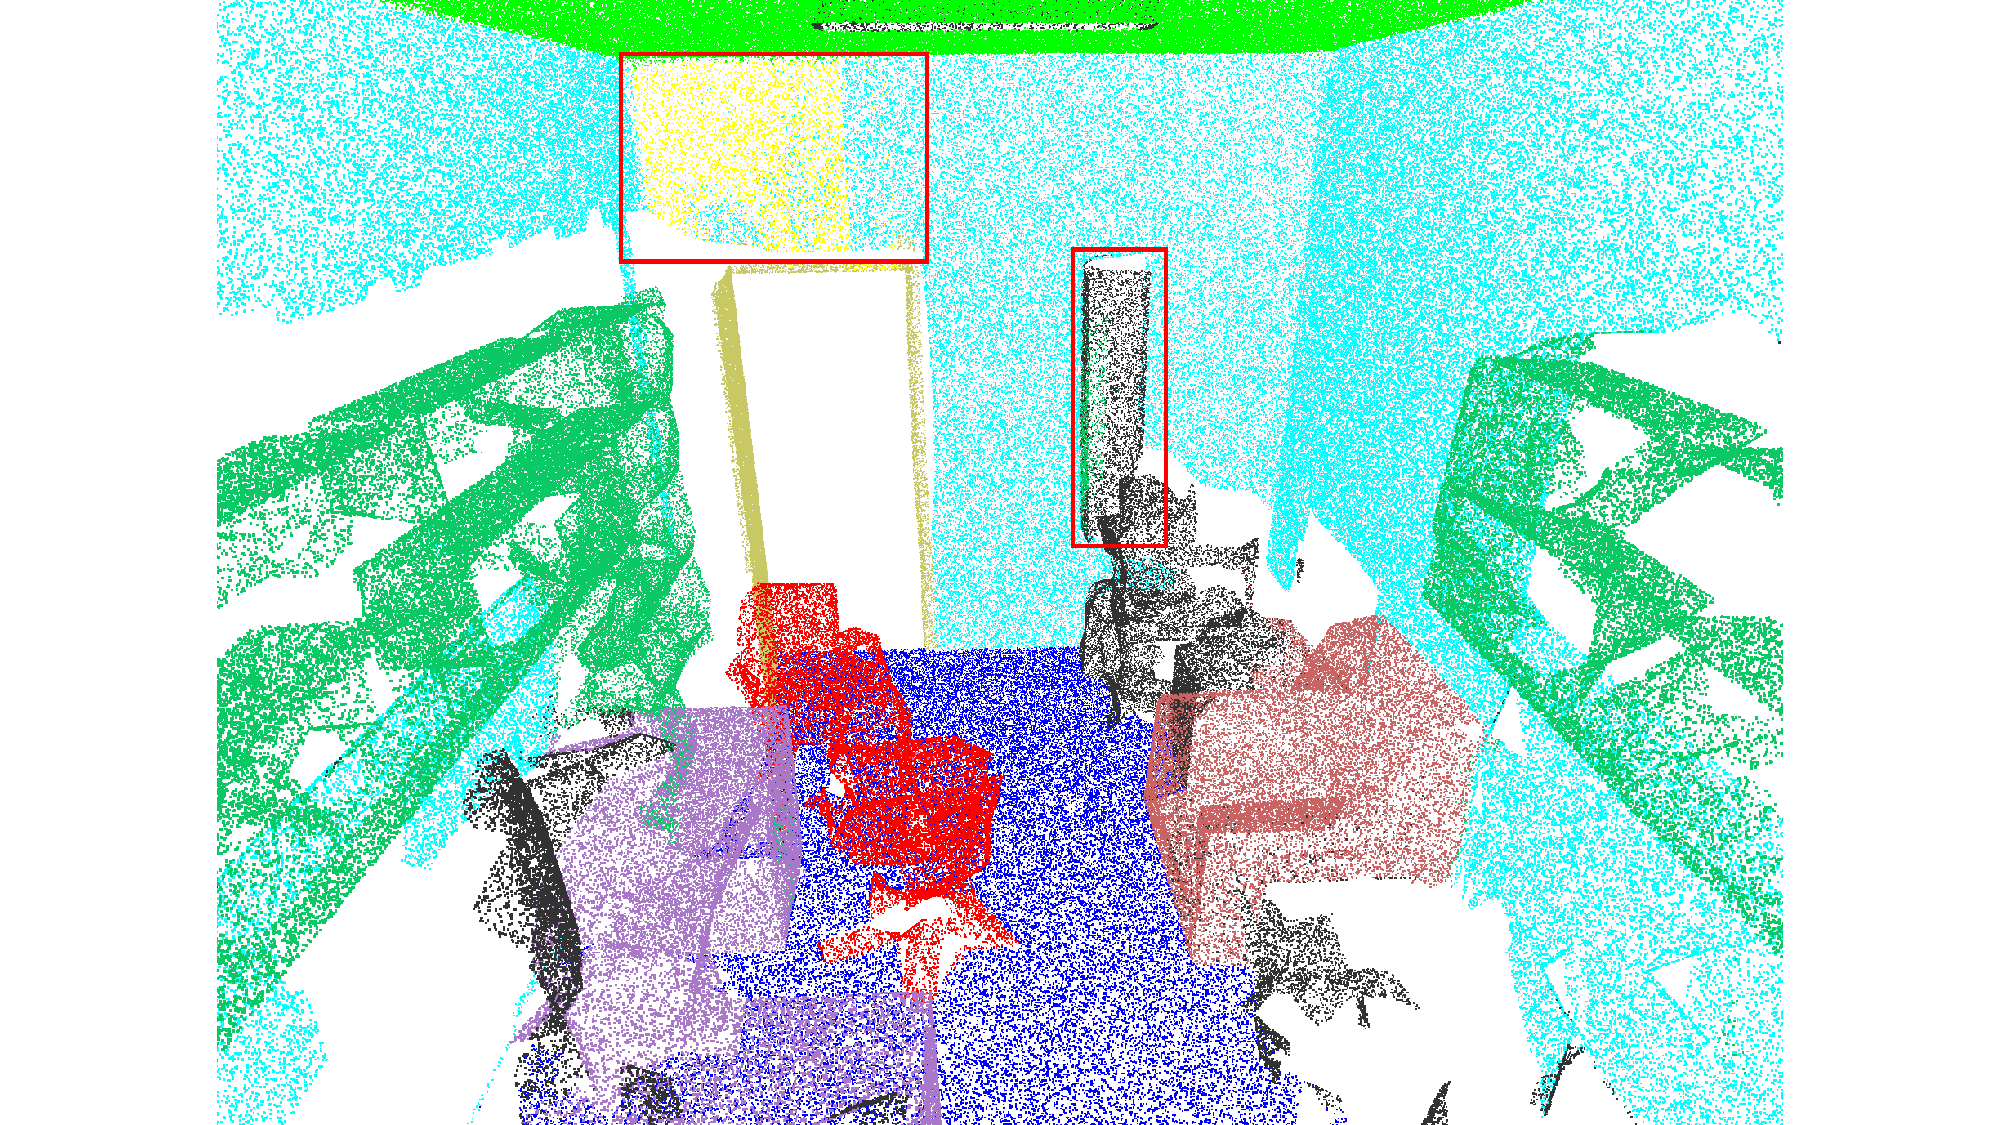
\includegraphics[width=\linewidth]{fig/S3DIS/DAPT.pdf}
        % \caption*{\textbf{\#TP}:1.7M \textbf{\#OA}:84.94}
        \caption{DAPT~\cite{zhou2024dynamic}}
        \label{fig:s3dis2}
    \end{subfigure}
    \hfill
    \begin{subfigure}{0.235\textwidth}
        \centering
        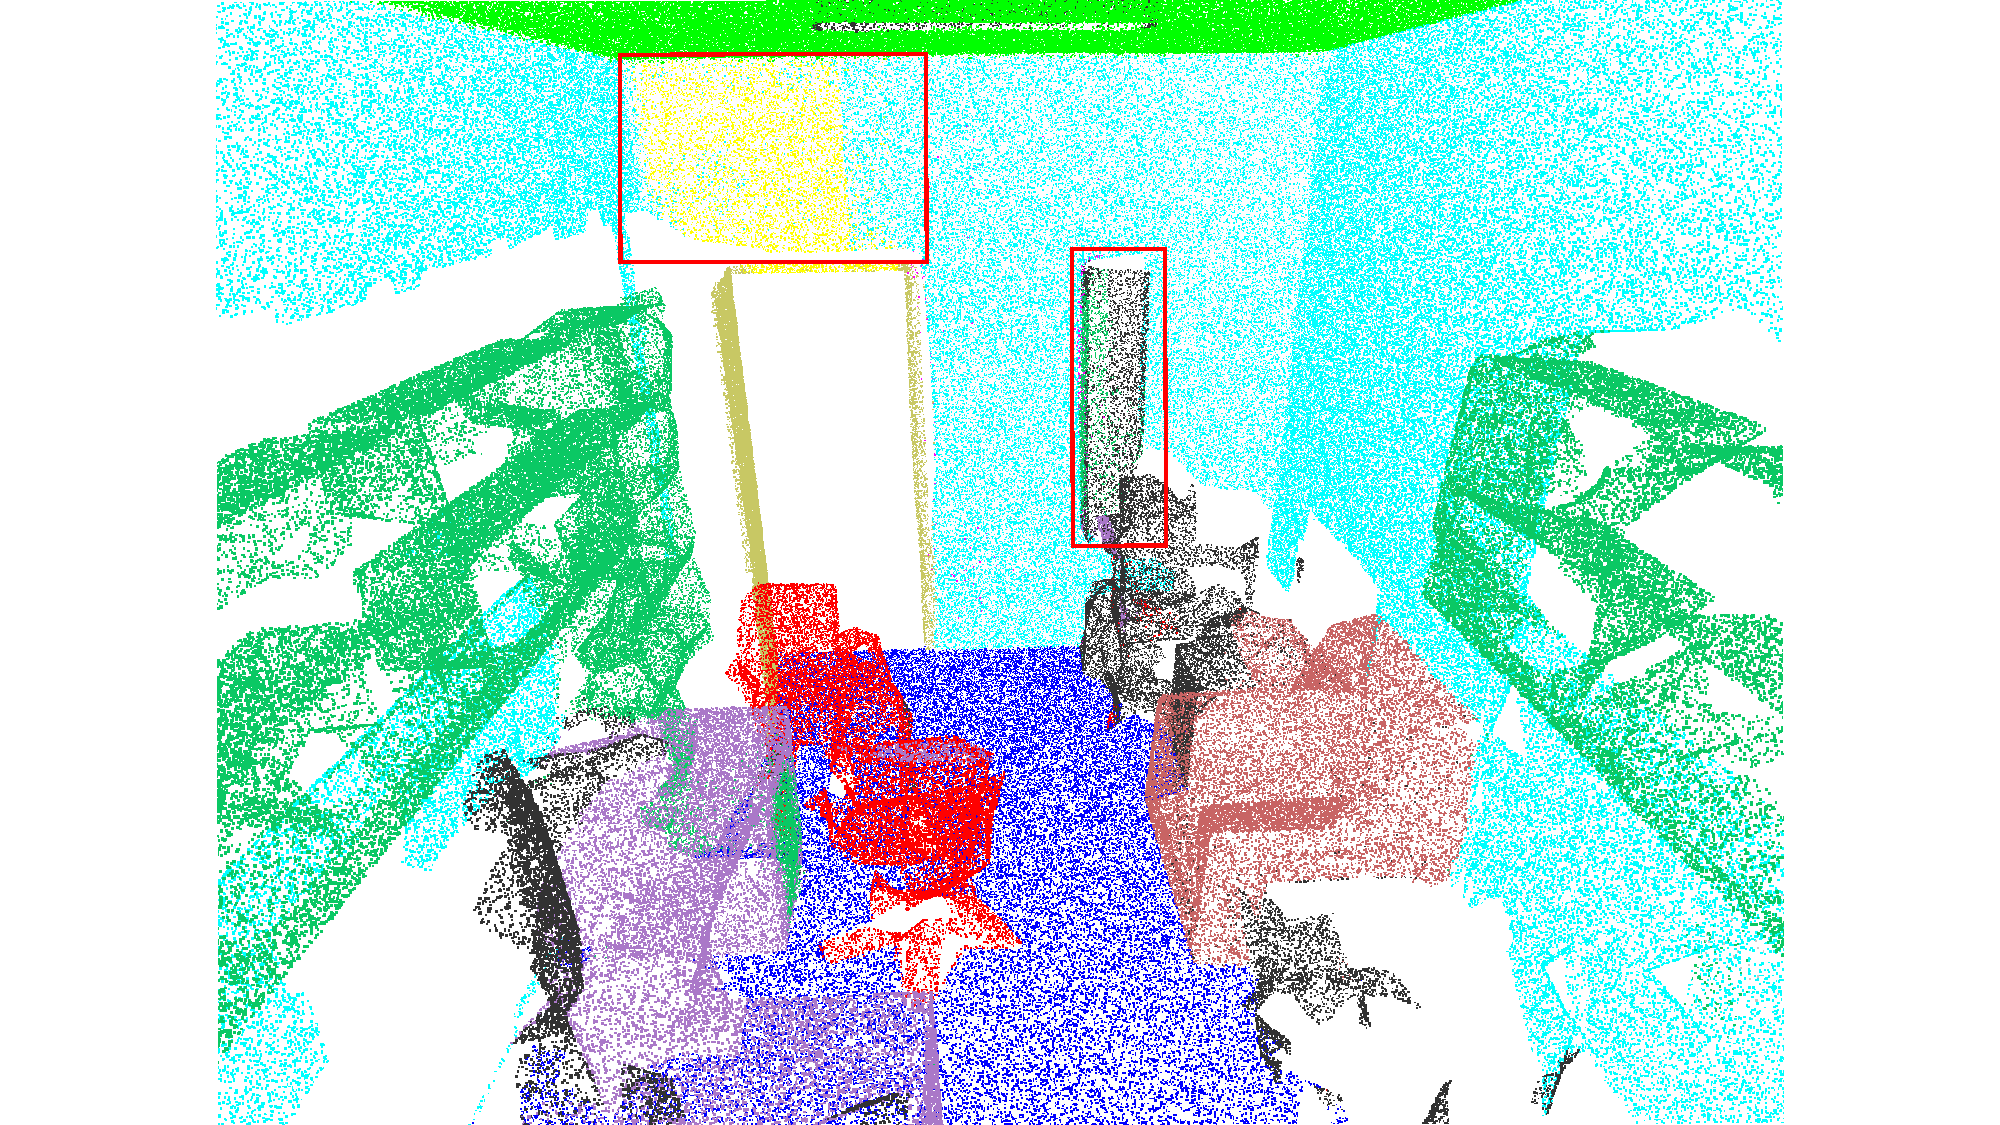
\includegraphics[width=\linewidth]{fig/S3DIS/IDPT.pdf}
        % \caption*{\textbf{\#TP}:1.1M \textbf{\#OA}:85.08}
        \caption{IDPT~\cite{zha2023instance}}
        \label{fig:s3dis3}
    \end{subfigure}
    \hfill
    \begin{subfigure}{0.235\textwidth}
        \centering
        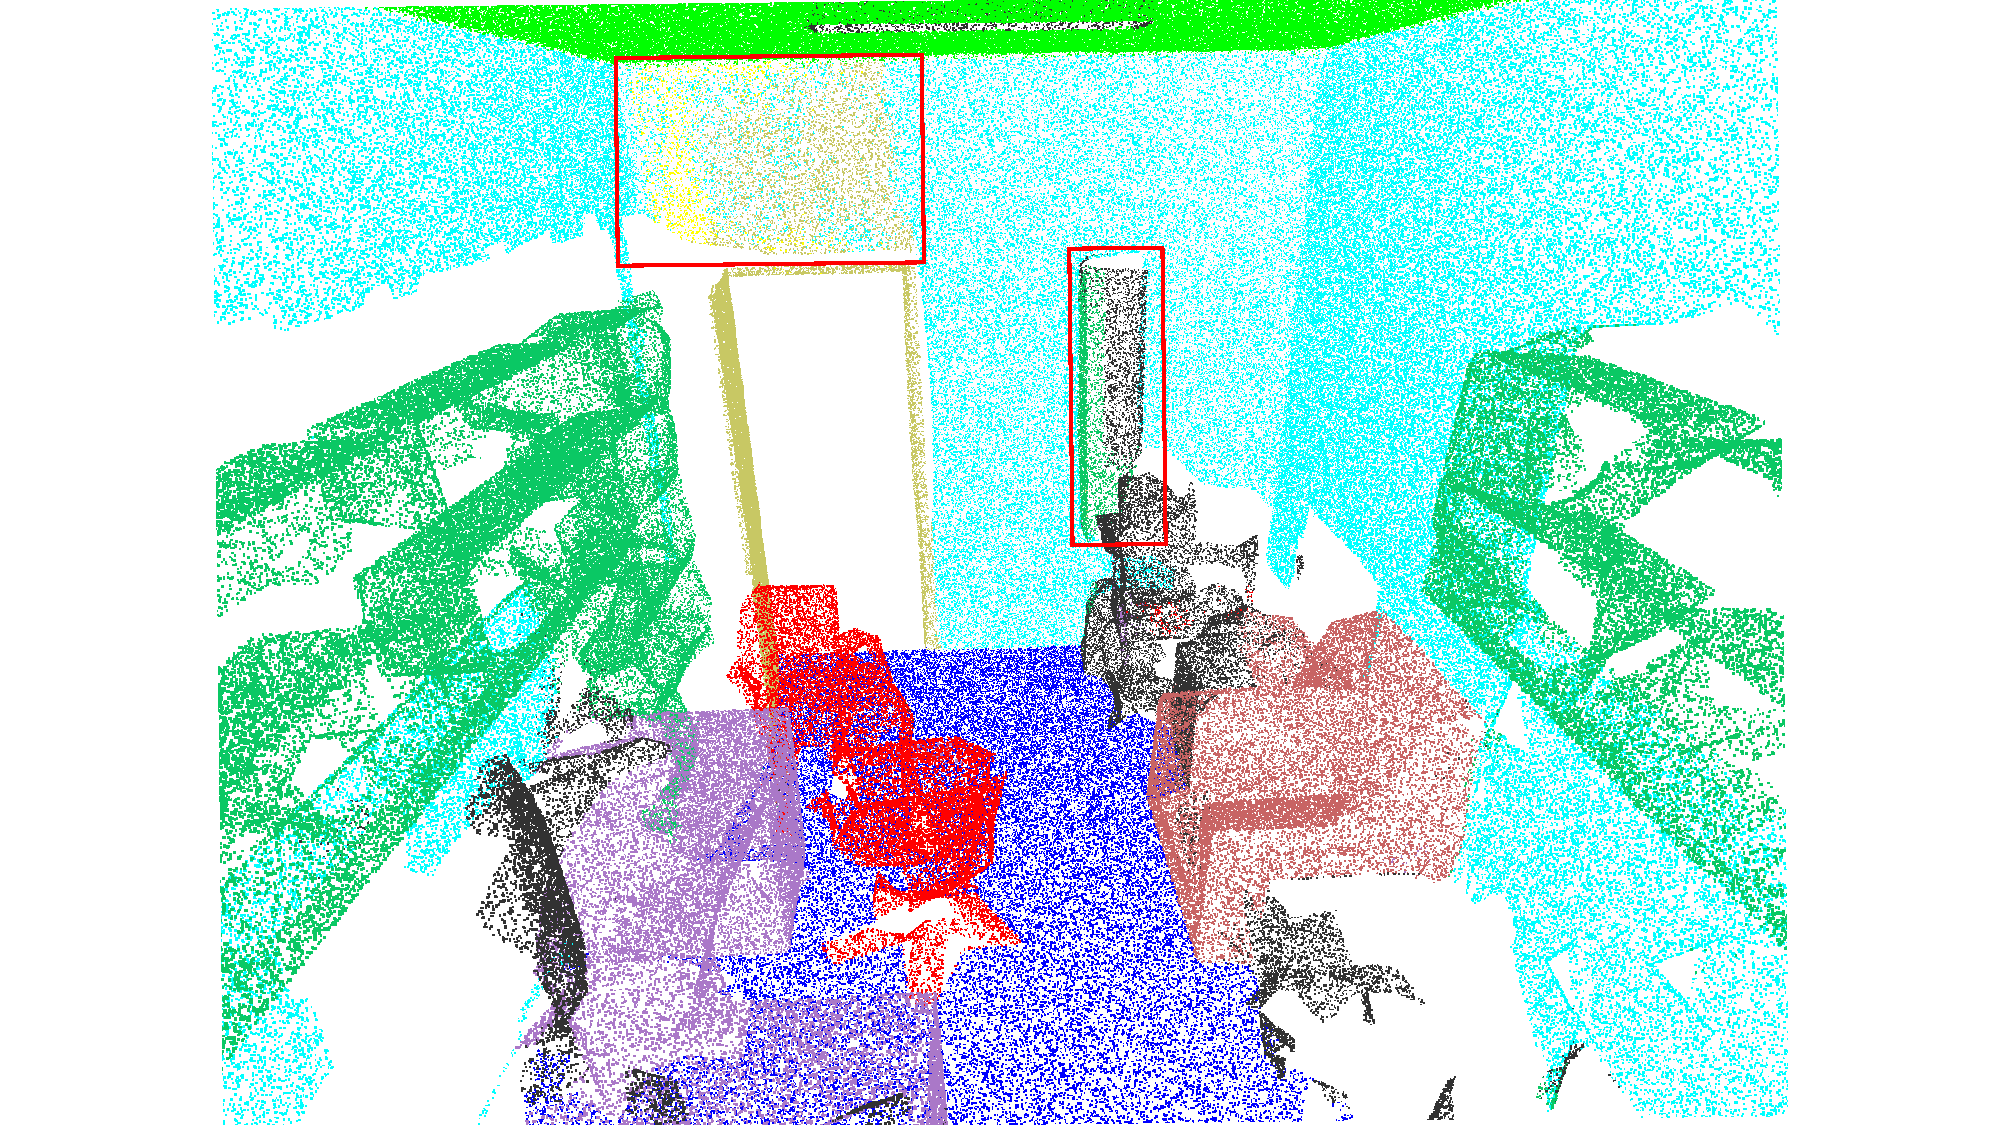
\includegraphics[width=\linewidth]{fig/S3DIS/PPT.pdf}
        % \caption*{\textbf{\#TP}:1.1M \textbf{\#OA}:84.91}
        \caption{PPT~\cite{zhang2024positional}}
        \label{fig:s3dis4}
    \end{subfigure}
    \hfill
    \begin{subfigure}{0.235\textwidth}
        \centering
        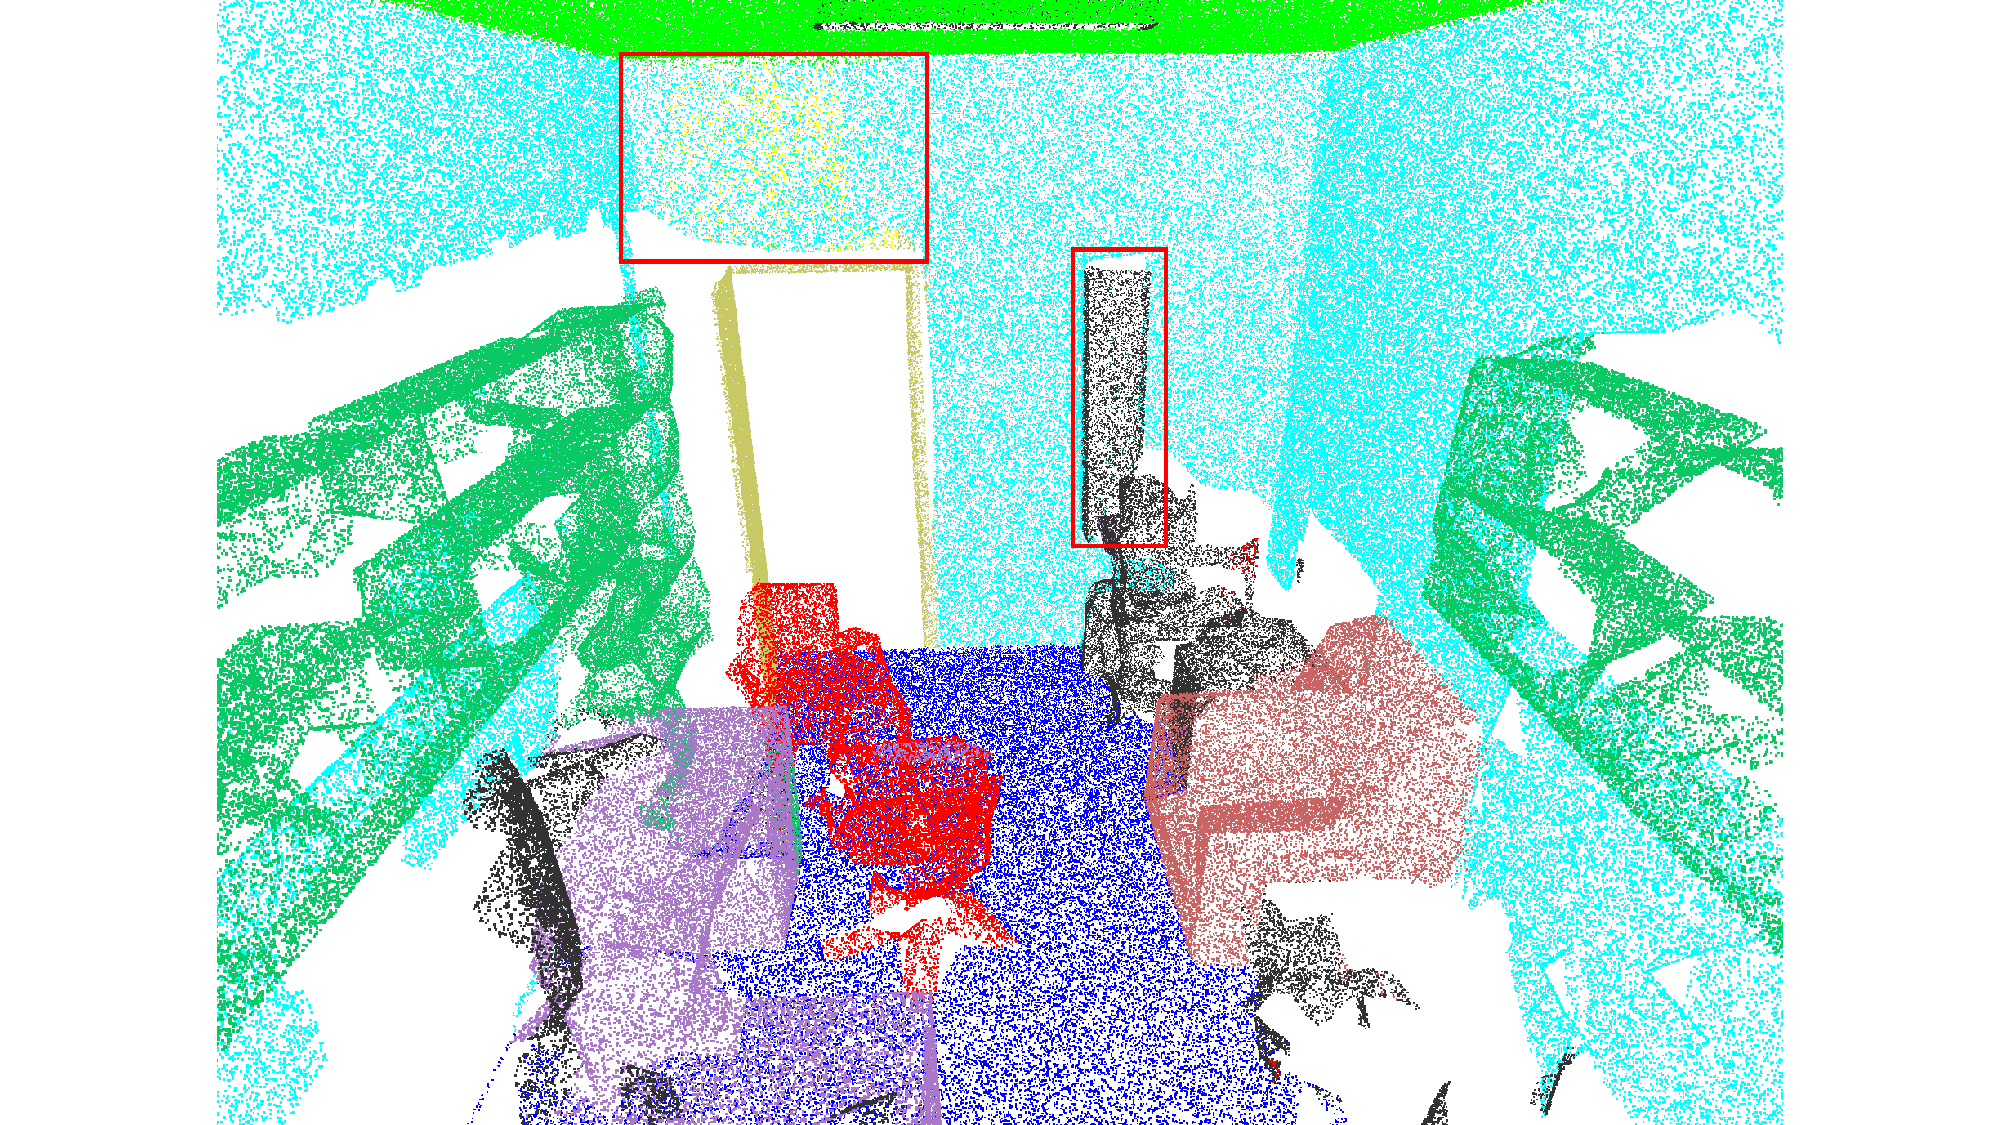
\includegraphics[width=\linewidth]{fig/S3DIS/PLT.pdf}
        % \caption*{\textbf{\#TP}:0.8M \textbf{\#OA}:82.75}
        \caption{PLT (Ours)}
        \label{fig:s3dis5}
    \end{subfigure}
    \hfill
    \begin{subfigure}{0.235\textwidth}
        \centering
        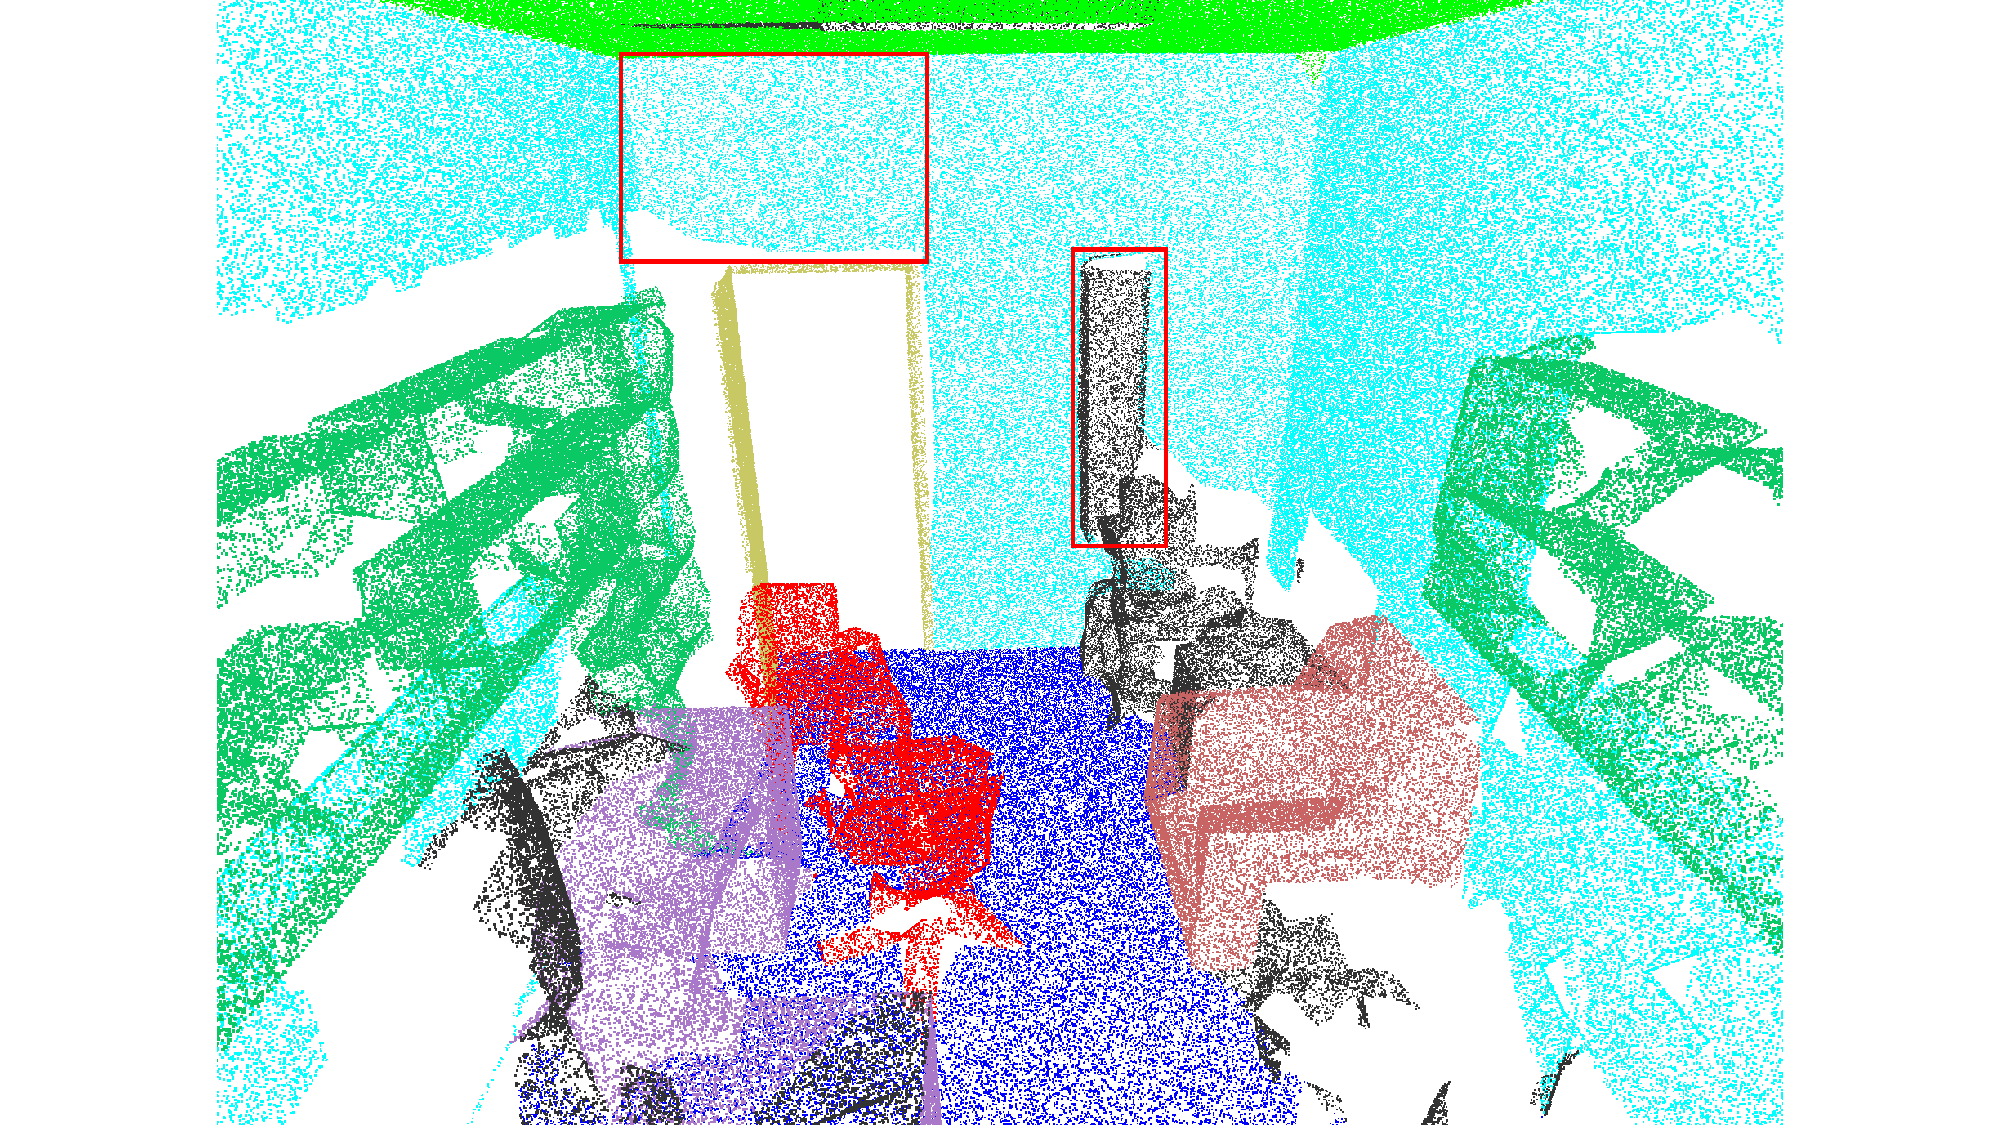
\includegraphics[width=\linewidth]{fig/S3DIS/GT.pdf}
        % \caption*{\textbf{\#TP}:0.6M \textbf{\#OA}:85.46}
        \caption{GT}
        \label{fig:s3dis6}
    \end{subfigure}
    \caption{The visualizations from the Area5 of S3DIS using a pre-trained PointMAE with different fine-tuning strategies.}
    \label{fig:s3dis}
\end{figure}
\begin{figure*}
    \centering
    \begin{subfigure}{0.19\textwidth}
        \centering
        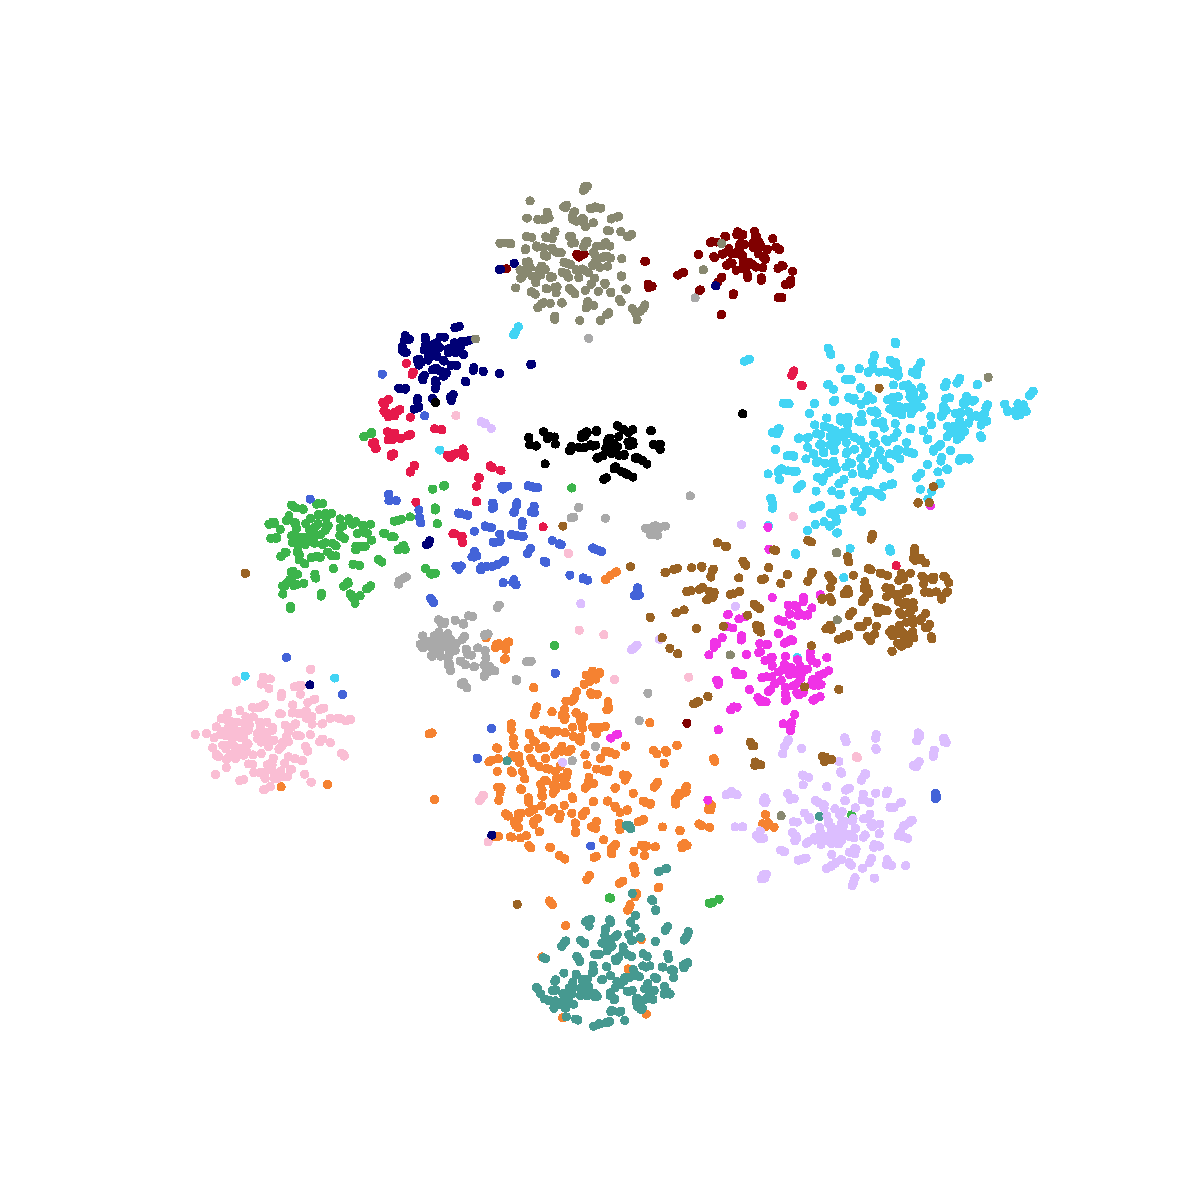
\includegraphics[width=\linewidth]{fig/tsne/point_mae.pdf}
        \caption*{\textbf{\#TP}:22.1M \textbf{\#OA}:85.18}
        \caption{Full fine-tuning}
        \label{fig:sub1}
    \end{subfigure}
    \hfill
    \begin{subfigure}{0.19\textwidth}
        \centering
        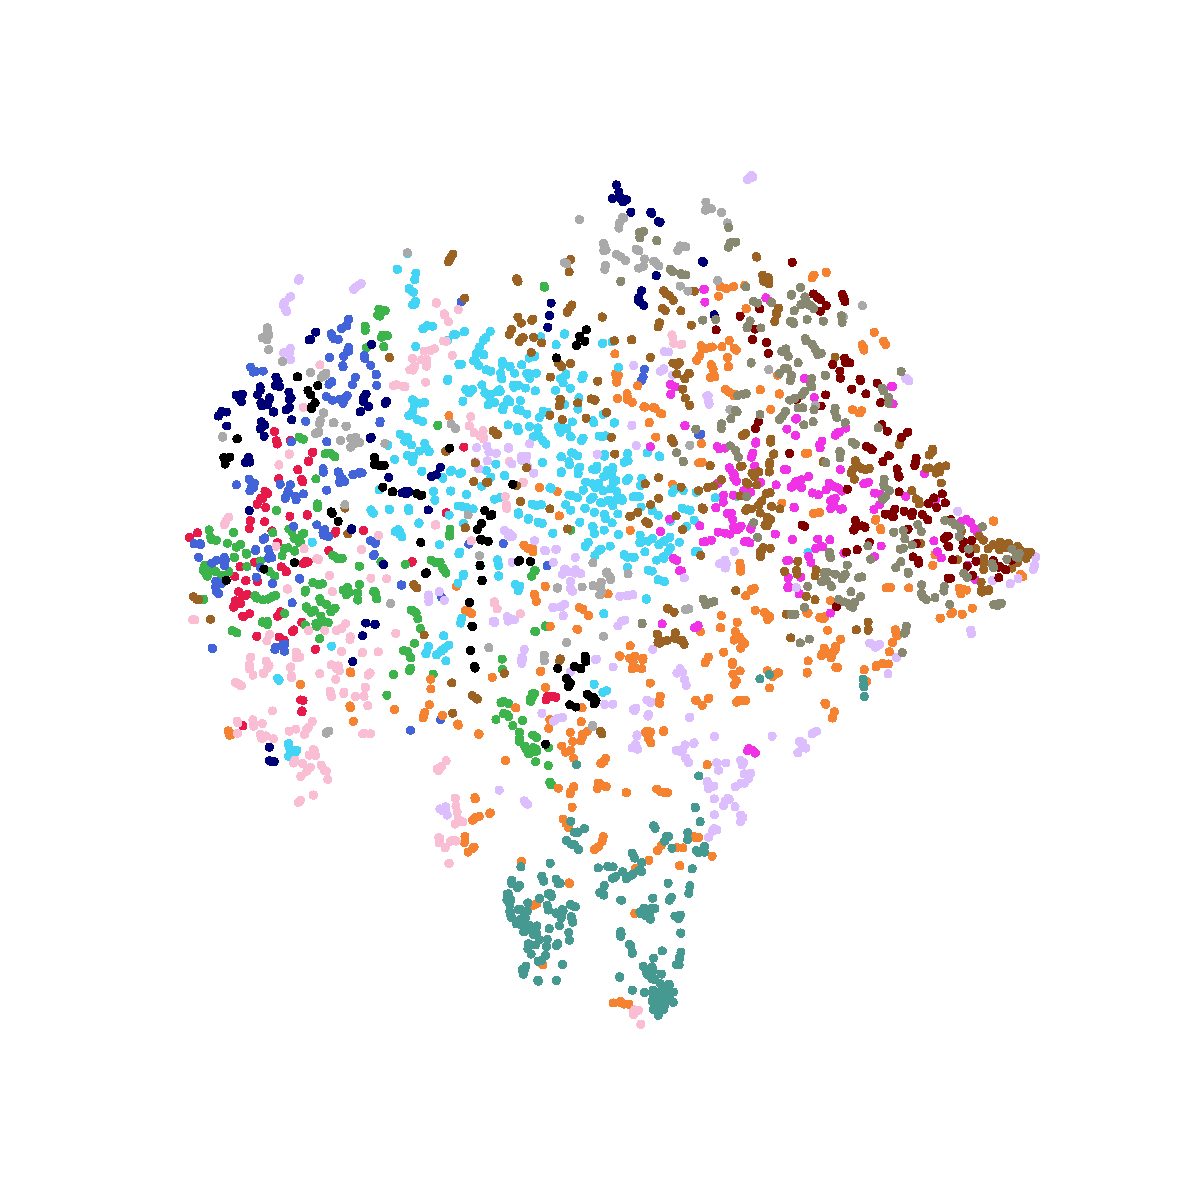
\includegraphics[width=\linewidth]{fig/tsne/LP.pdf}
        \caption*{\textbf{\#TP}:0.3M \textbf{\#OA}:75.99}
        \caption{Linear Probing}
        \label{fig:sub2}
    \end{subfigure}
    \hfill
    \begin{subfigure}{0.19\textwidth}
        \centering
        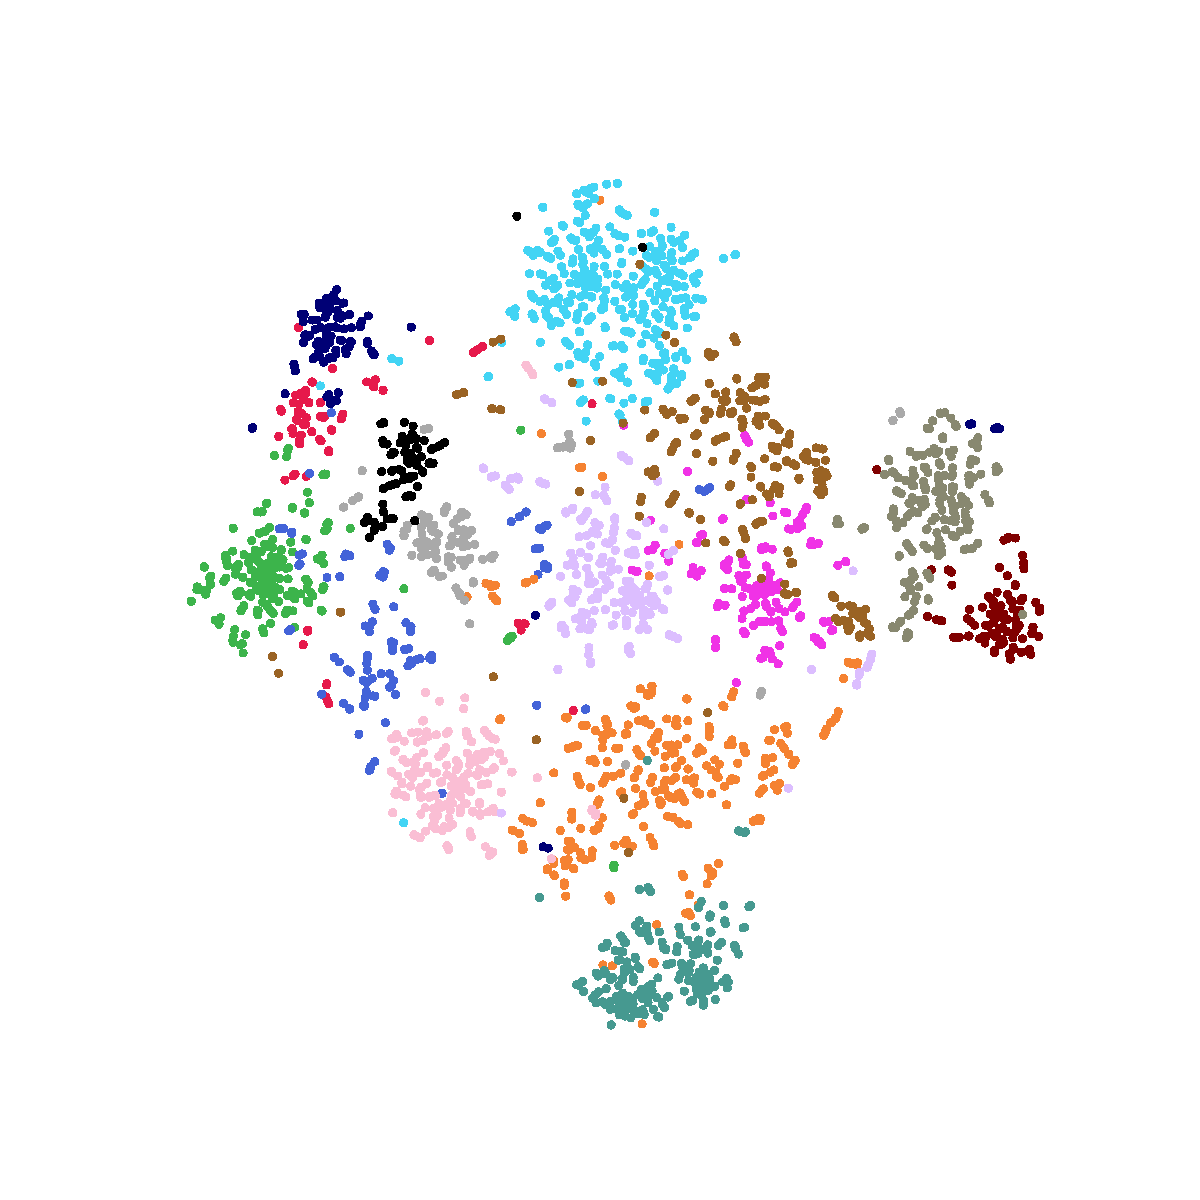
\includegraphics[width=\linewidth]{fig/tsne/idpt.pdf}
        \caption*{\textbf{\#TP}:1.7M \textbf{\#OA}:84.94}
        \caption{IDPT}
        \label{fig:sub3}
    \end{subfigure}
    \hfill
    \begin{subfigure}{0.19\textwidth}
        \centering
        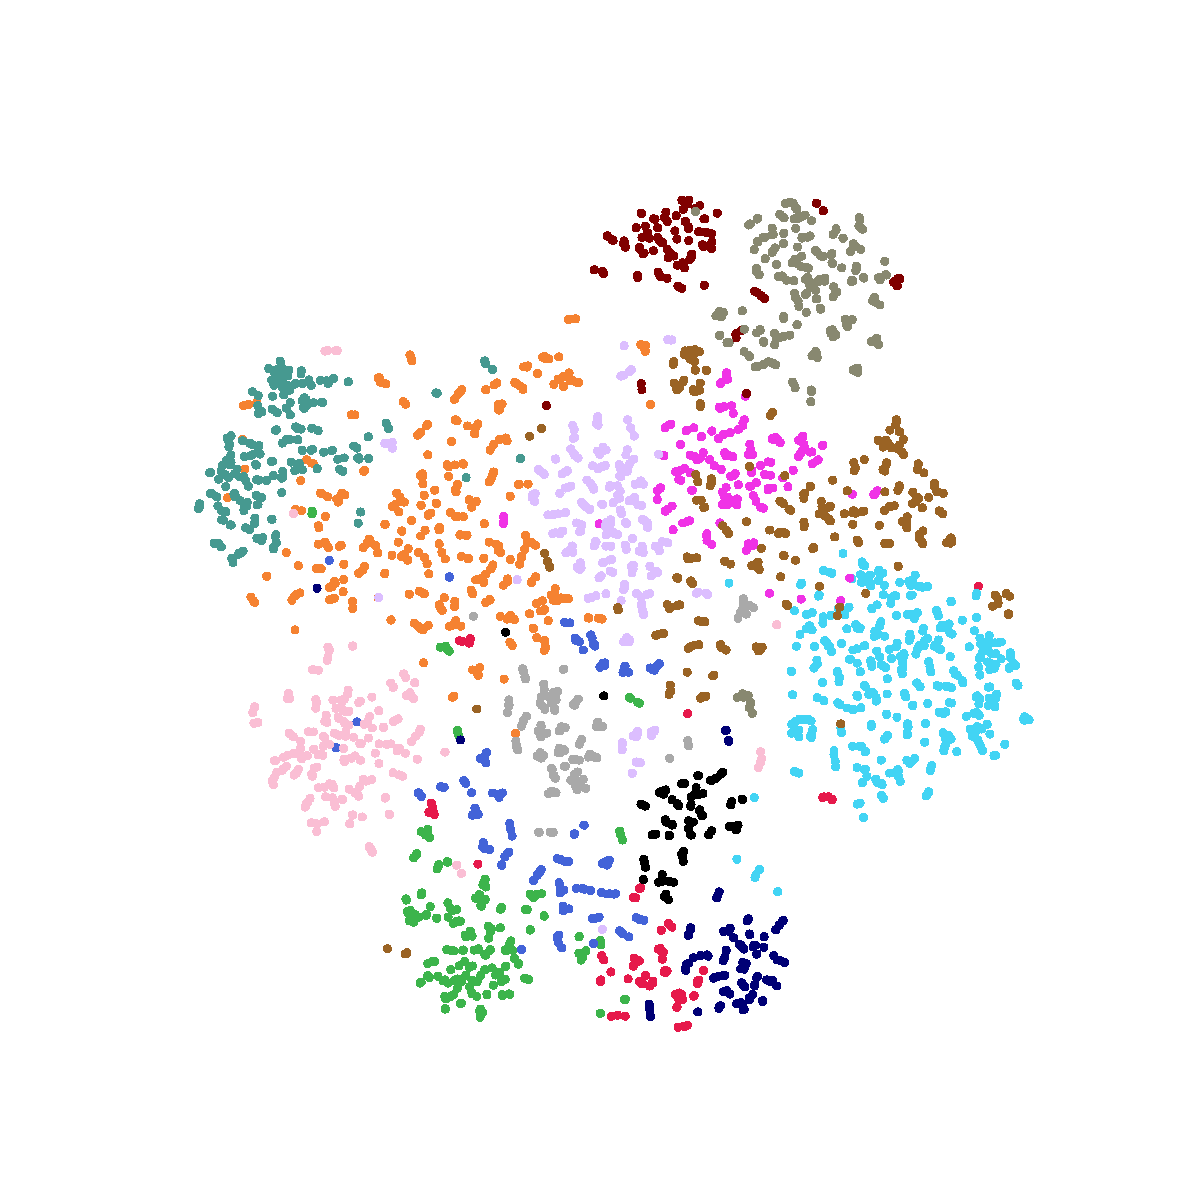
\includegraphics[width=\linewidth]{fig/tsne/dapt.pdf}
        \caption*{\textbf{\#TP}:1.1M \textbf{\#OA}:85.08}
        \caption{DAPT}
        \label{fig:sub4}
    \end{subfigure}
    % \hfill
    % \begin{subfigure}{0.24\textwidth}
    %     \centering
    %     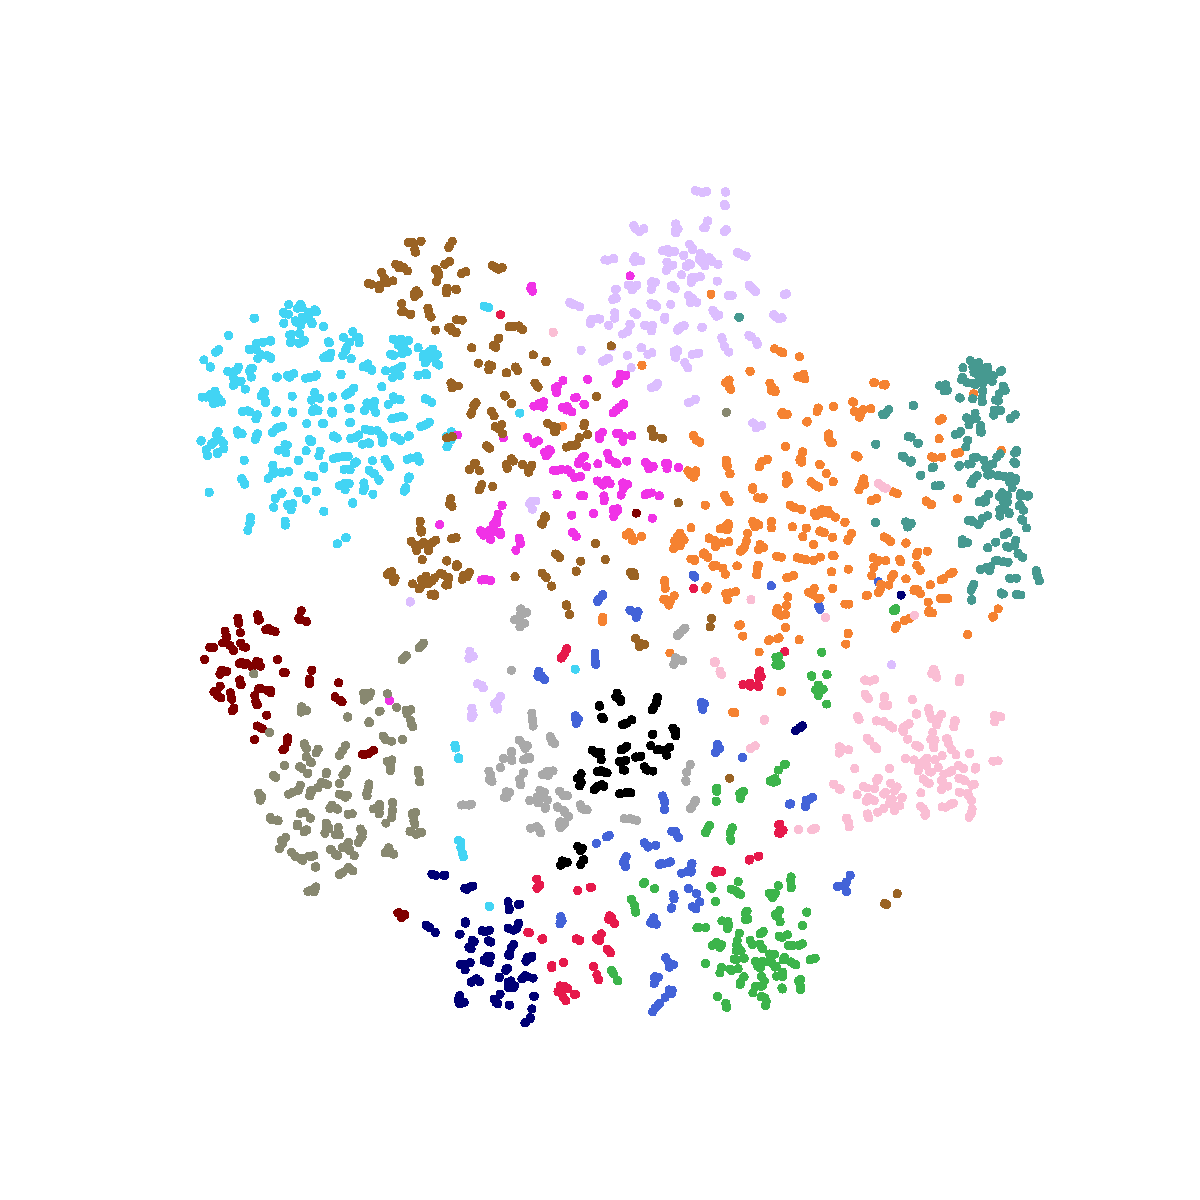
\includegraphics[width=\linewidth]{fig/tsne/pointgst.pdf}
    %     \caption*{\textbf{\#TP}:0.6M \textbf{\#OA}:85.29}
    %     \caption{PointGST}
    %     \label{fig:sub5}
    % \end{subfigure}
    % \hfill
    % \begin{subfigure}{0.24\textwidth}
    %     \centering
    %     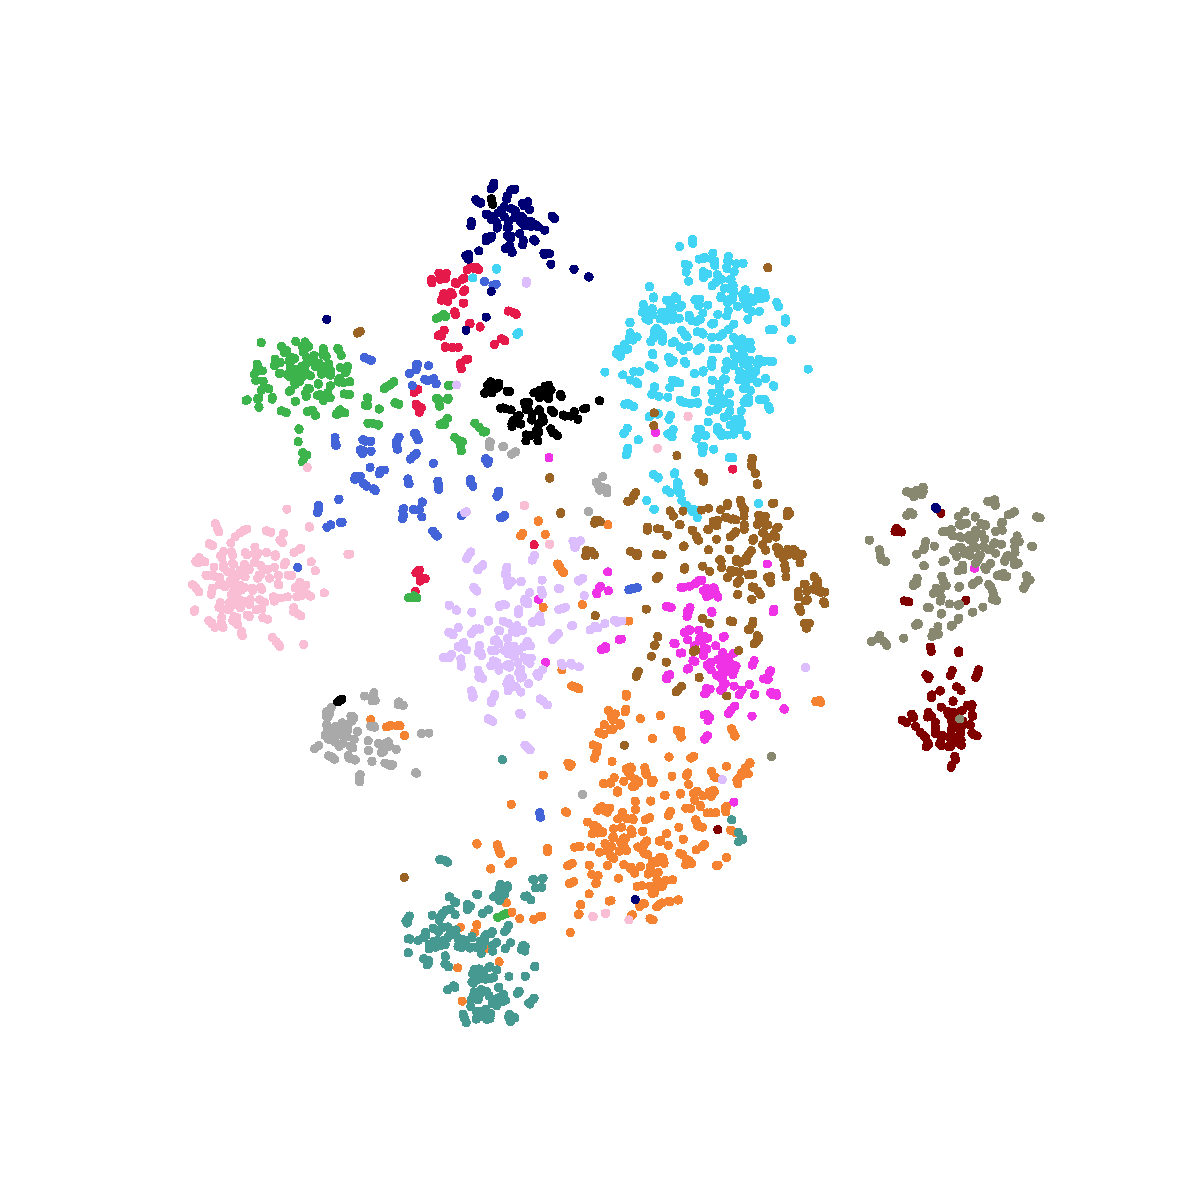
\includegraphics[width=\linewidth]{fig/tsne/PPT.pdf}
    %     \caption*{\textbf{\#TP}:1.1M \textbf{\#OA}:84.91}
    %     \caption{PPT}
    %     \label{fig:sub6}
    % \end{subfigure}
    % \hfill
    % \begin{subfigure}{0.24\textwidth}
    %     \centering
    %     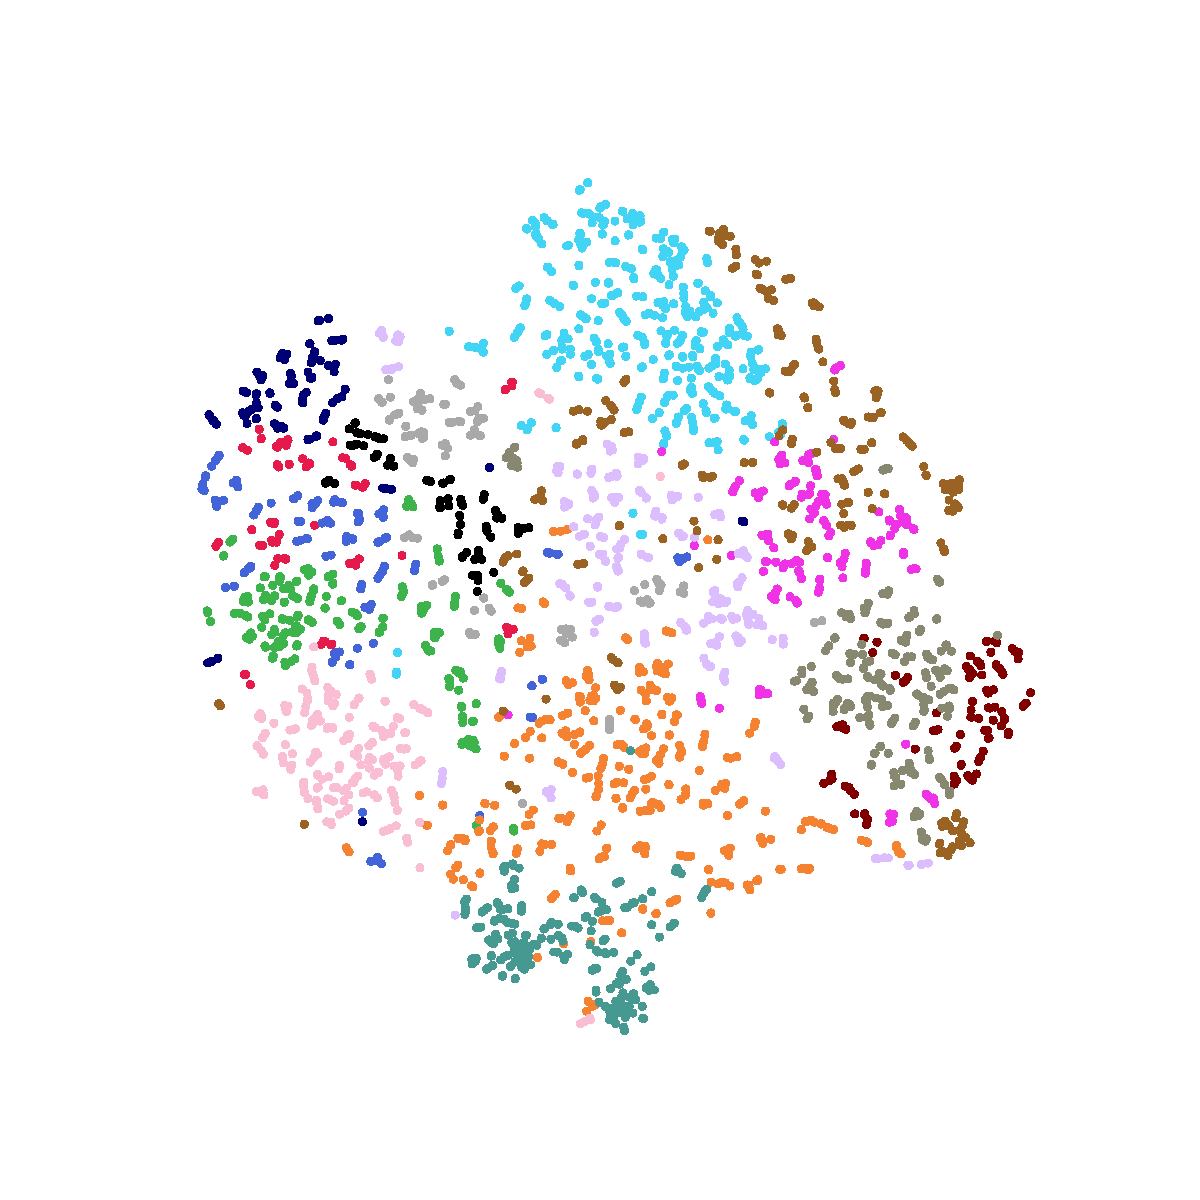
\includegraphics[width=\linewidth]{fig/tsne/LST.pdf}
    %     \caption*{\textbf{\#TP}:0.8M \textbf{\#OA}:82.75}
    %     \caption{LST}
    %     \label{fig:sub7}
    % \end{subfigure}
    \hfill
    \begin{subfigure}{0.19\textwidth}
        \centering
        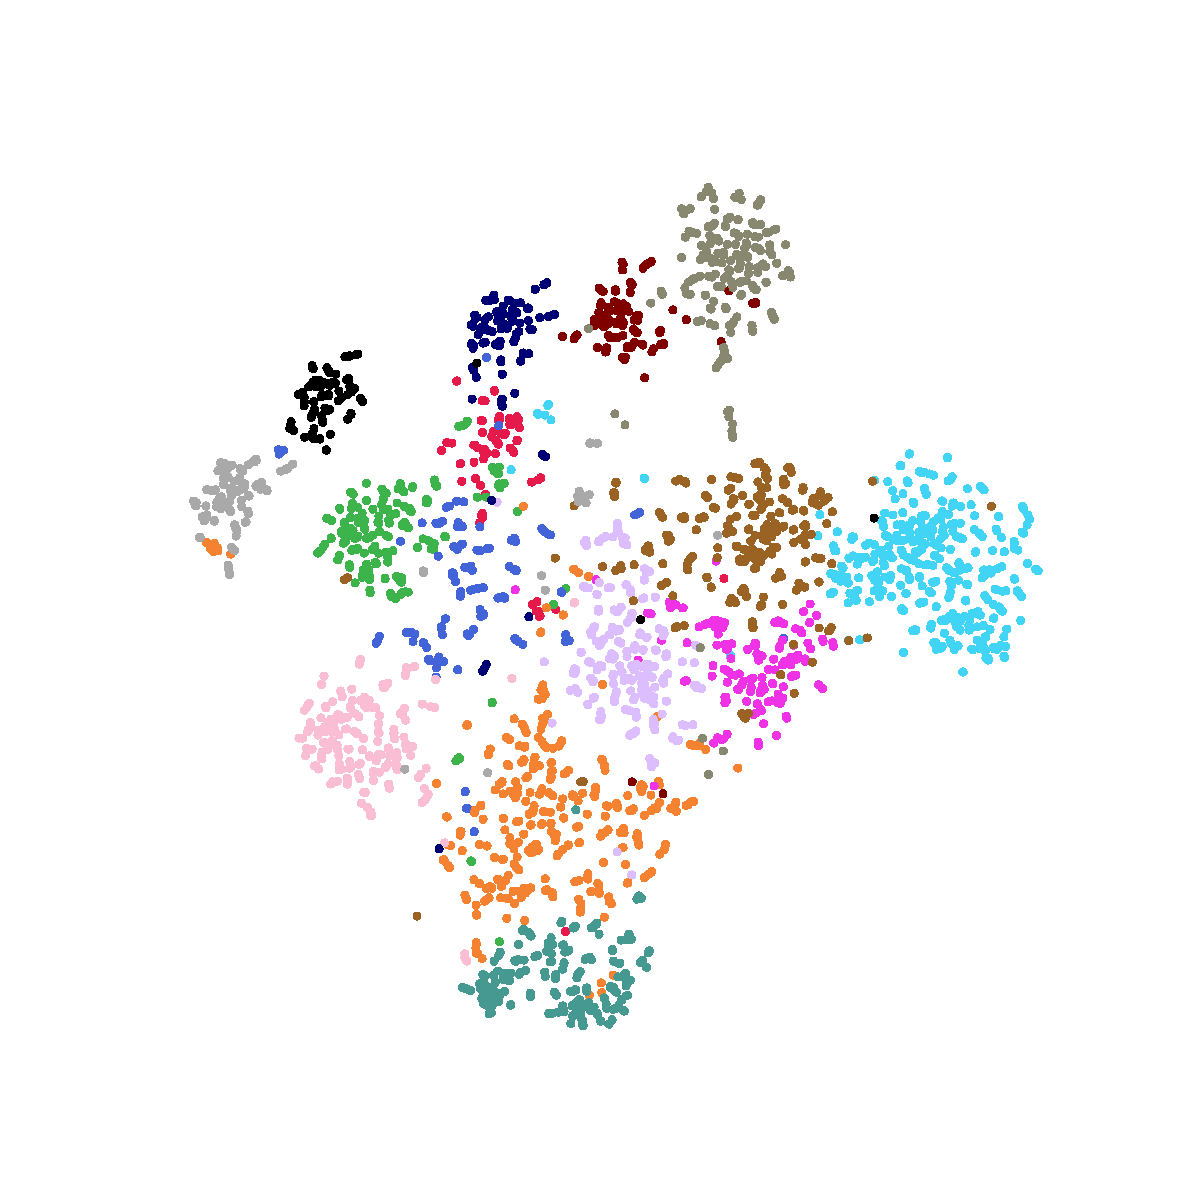
\includegraphics[width=\linewidth]{fig/tsne/point_ladder.pdf}
        \caption*{\textbf{\#TP}:0.6M \textbf{\#OA}:85.53}
        \caption{PLT (Ours)}
        \label{fig:sub8}
    \end{subfigure}
    \caption{The visualization of the t-SNE~\cite{van2008visualizing} from the test sets of ScanObjectNN~\cite{uy2019revisiting} (PB\_T50\_RS) by using a pre-trained PointMAE~\cite{pang2022masked} with various fine-tuning strategies. We extract the final classification features from the top linear layer for t-SNE visualizations.}
    \label{fig:tsne}
\end{figure*}

\subsection{Performance Analysis}

Tab.\ref{tab:performance} provides a comprehensive comparison of our PLT framework against various recent parameter-efficient tuning methods built upon the Point-MAE\cite{pang2022masked} baseline. The evaluation is conducted on the most challenging variant of ScanObjectNN~\cite{uy2019revisiting} (i.e., PB\_T50\_RS), with consistent settings including a batch size of 32 and all throughput metrics measured on a single NVIDIA RTX 3090 GPU.

Our method achieves the best accuracy (85.53\%) among all competing approaches, outperforming the original full fine-tuning baseline (85.18\%) and other prompt tuning or adapter-based methods. Notably, PLT accomplishes this with only 0.60M trainable parameters—merely 2.7\% of the full Point-MAE model—demonstrating remarkable parameter efficiency. In comparison, methods such as IDPT~\cite{zha2023instance} (1.70M) and DAPT~\cite{zhou2024dynamic} (1.09M) use significantly more parameters while yielding inferior accuracy.

In terms of computational complexity, PLT maintains a moderate FLOPs level (5.02GFLOPs), comparable to the baseline PointMAE~\cite{pang2022masked} (4.93GFLOPs) and much lower than IDPT~\cite{zha2023instance} (7.27GFLOPs), further validating its lightweight design. From a practical deployment standpoint, PLT achieves favorable training throughput (165.4 samples/s) and inference speed (210.8 samples/s), striking a solid balance between speed and effectiveness. While DAPT offers slightly higher training throughput (169.0 samples/s), its accuracy and parameter efficiency are not as competitive.

%Memory usage is also a critical factor. PLT maintains low inference memory (0.85G), on par with most methods and substantially better than PointPEFT~\cite{tang2024point} (1.12G). Although the incorporation of FPS and KNN operations in PLT leads to a moderate increase in training memory consumption (2.26G), the overhead remains acceptable in practical applications. Notably, PLT still maintains a significantly lower memory footprint compared to other methods (e.g. PointPEFT~\cite{tang2024point} (8.64G) and IDPT~\cite{zha2023instance} (5.10G)) that also rely on similar operations.

Memory efficiency is another key advantage of PLT. During inference, PLT maintains a low memory footprint (0.85GB), comparable to most methods and significantly better than PointPEFT~\cite{tang2024point} (1.12GB). While training memory increases moderately to 2.26GB due to FPS and KNN operations, this remains practical and is still substantially lower than alternatives like PointPEFT (8.64GB) and IDPT~\cite{zha2023instance} (5.10GB) that use similar operations.

Overall, PLT demonstrates strong performance across all dimensions—achieving top-tier accuracy with minimal parameters, competitive FLOPs, efficient inference and training speeds, and modest memory consumption. This highlights its suitability for real-world deployment where both effectiveness and efficiency are essential. Importantly, PLT achieves this without sacrificing the backbone architecture or requiring extensive architectural re-design, offering a plug-and-play solution compatible with powerful pretrained models like Point-MAE~\cite{pang2022masked}.